%%%%%%%%%%%%%%%%%%%%%%%%%%%%%%%%%%%%%%%%%
% Beamer Presentation
% LaTeX Template
% Version 1.0 (10/11/12)
%
% This template has been downloaded from:
% http://www.LaTeXTemplates.com
%
% License:
% CC BY-NC-SA 3.0 (http://creativecommons.org/licenses/by-nc-sa/3.0/)
%
%%%%%%%%%%%%%%%%%%%%%%%%%%%%%%%%%%%%%%%%%

%----------------------------------------------------------------------------------------
%	PACKAGES AND THEMES
%----------------------------------------------------------------------------------------
\documentclass{beamer}
\usepackage{tikz}
\usetikzlibrary{fadings}

\mode<presentation> {

% The Beamer class comes with a number of default slide themes
% which change the colors and layouts of slides. Below this is a list
% of all the themes, uncomment each in turn to see what they look like.

%\usetheme{default}
%\usetheme{AnnArbor}
%\usetheme{Antibes}
%\usetheme{Bergen}
%\usetheme{Berkeley}
%\usetheme{Berlin}
%\usetheme{Boadilla}
%\usetheme{CambridgeUS}
%\usetheme{Copenhagen}
%\usetheme{Darmstadt}
%\usetheme{Dresden}
%\usetheme{Frankfurt}
%\usetheme{Goettingen}
%\usetheme{Hannover}
%\usetheme{Ilmenau}
%\usetheme{JuanLesPins}
%\usetheme{Luebeck}
\usetheme{Madrid}
%\usetheme{Malmoe}
%\usetheme{Marburg}
%\usetheme{Montpellier}
%\usetheme{PaloAlto}
%\usetheme{Pittsburgh}
%\usetheme{Rochester}
%\usetheme{Singapore}
%\usetheme{Szeged}
%\usetheme{Warsaw}

% As well as themes, the Beamer class has a number of color themes
% for any slide theme. Uncomment each of these in turn to see how it
% changes the colors of your current slide theme.

%\usecolortheme{albatross}
%\usecolortheme{beaver}
%\usecolortheme{beetle}
%\usecolortheme{crane}
%\usecolortheme{dolphin}
%\usecolortheme{dove}
%\usecolortheme{fly}
%\usecolortheme{lily}
%\usecolortheme{orchid}
%\usecolortheme{rose}
%\usecolortheme{seagull}
%\usecolortheme{seahorse}
%\usecolortheme{whale}
%\usecolortheme{wolverine}

%\setbeamertemplate{footline} % To remove the footer line in all slides uncomment this line
%\setbeamertemplate{footline}[page number] % To replace the footer line in all slides with a simple slide count uncomment this line
\setbeamertemplate{caption}{\raggedright\insertcaption\par}
\setbeamertemplate{navigation symbols}{} % To remove the navigation symbols from the bottom of all slides uncomment this line
}
\usepackage{siunitx}
\usepackage{graphicx} % Allows including images
\usepackage{tikz}
\usepackage{pgfplots}
\usepackage{booktabs} % Allows the use of \toprule, \midrule and \bottomrule in tables
\usepackage{sidecap}
\definecolor{links}{HTML}{2A1B81}
\hypersetup{colorlinks,linkcolor=,urlcolor=links}
\hypersetup{urlcolor=links}

%----------------------------------------------------------------------------------------
%	TITLE PAGE
%----------------------------------------------------------------------------------------

\title[EUTelescope and GBL]{The GBL Tracking Algorithm in EUTelescope} % The short title appears at the bottom of every slide, the full title is only on the title page

\author{Alexander Morton} % Your name
\institute[Glasgow] % Your institution as it will appear on the bottom of every slide, may be shorthand to save space
{
University of Glasgow \\ % Your institution for the title page
\medskip
\textit{a.morton.2@research.com} % Your email address
}
\date{\today} % Date, can be changed to a custom date

\logo{
\includegraphics[scale = 0.025]{pics/GlaUni.png}}
\titlegraphic{

\includegraphics[scale = 0.2]{pics/EUTel.png}\\

\includegraphics[scale = 0.2]{pics/gbl-logo.png}

\includegraphics[scale = 0.2]{pics/mp2-logo.png}
}
\begin{document}

\begin{frame}
\titlepage % Print the title page as the first slide
\end{frame}

%\begin{frame}
%\frametitle{Overview} % Table of contents slide, comment this block out to remove it
%\tableofcontents % Throughout your presentation, if you choose to use \section{} and \subsection{} commands, these will automatically be printed on this slide as an overview of your presentation
%\end{frame}
%----------------------------------------------------------------------------------------
%	PRESENTATION SLIDES
%----------------------------------------------------------------------------------------

%------------------------------------------------


%------------------------------------------------
\section{Track Fitting in EUTelescope}
\subsection{EUDET/AIDA Pixel Beam Telescope}
\begin{frame}
\frametitle{EUDET/AIDA Pixel Beam Telescope}
\begin{itemize}
\small{
\item The telescope is a series of pixel sensors used to reconstruct particle trajectories
\item To reconstruct a particles trajectory the position/time must be determined with the following 
\begin{enumerate}
\item  6 CMOS pixel detectors $\rightarrow$ 18.4x18.4 \si{\micro\metre\squared}  , 115.2 \si{\micro\second} integration time/frame.
\item Additional timing plane used in efficiency measurements to reduce the time resolution to 25 ns.
\end{enumerate}
\item EUTelescope is a reconstruction framework for this setup.
}
\end{itemize}
\begin{figure}
  \begin{columns}
        \column{.3\linewidth}
        \includegraphics[scale=0.03]{pics/setup.JPG}
        \label{fig:example left}
        \column{.6\linewidth}
        \caption{The telescope setup composed of 6 pixel sensors. }
      \end{columns}
\end{figure}
\end{frame}

\subsection{EUTelescope}
\begin{frame}
\frametitle{Track Reconstruction in EUTelescope}
\begin{itemize}
\item Broken lines track fitting is $\chi^{2}$ minimisation with scattering taken into consideration.
\item Two track fitting techniques are used at the moment.
\end{itemize}
\small{
\begin{enumerate}
\item Deterministic Annealing Filter $\rightarrow$ DAF. 
\begin{itemize}
\small{
\item Pattern recognition is combined with track fitting
\begin{itemize}
\item Does not allow addition of new pattern recognition methods. 
\end{itemize}
\item Models all scatterers as thin.
\item \textbf{Track fitting not possible with magnetic fields.} 
\item Usual method for track reconstruction
}
\end{itemize}
\item  General Broken Lines Algorithm $\rightarrow$ GBL
\begin{itemize}
\small{
\item A generic track fitting package written by Claus Kleinwort in C++.
\item Fit parameters are curvature and offsets. 
\item Scattering information is included in fit in the form of kink angles.
\item \textbf{Fitting with arbitrary magnetic fields.}
\item Easy to add additional track parameters of interest.
\begin{itemize}
\item X0 measurements use this feature
\end{itemize}
%\item First time use for testbeam reconstruction
}
\end{itemize}
\end{enumerate}
}
\textbf{A single track can be constructed in 4 steps...} 
\end{frame}
%------------------------------------------------

%------------------------------------------------
\subsection{Four Steps}
\begin{frame}
\frametitle{\textbf{1} The Discrete Track}
\begin{figure}
\label{Scat}
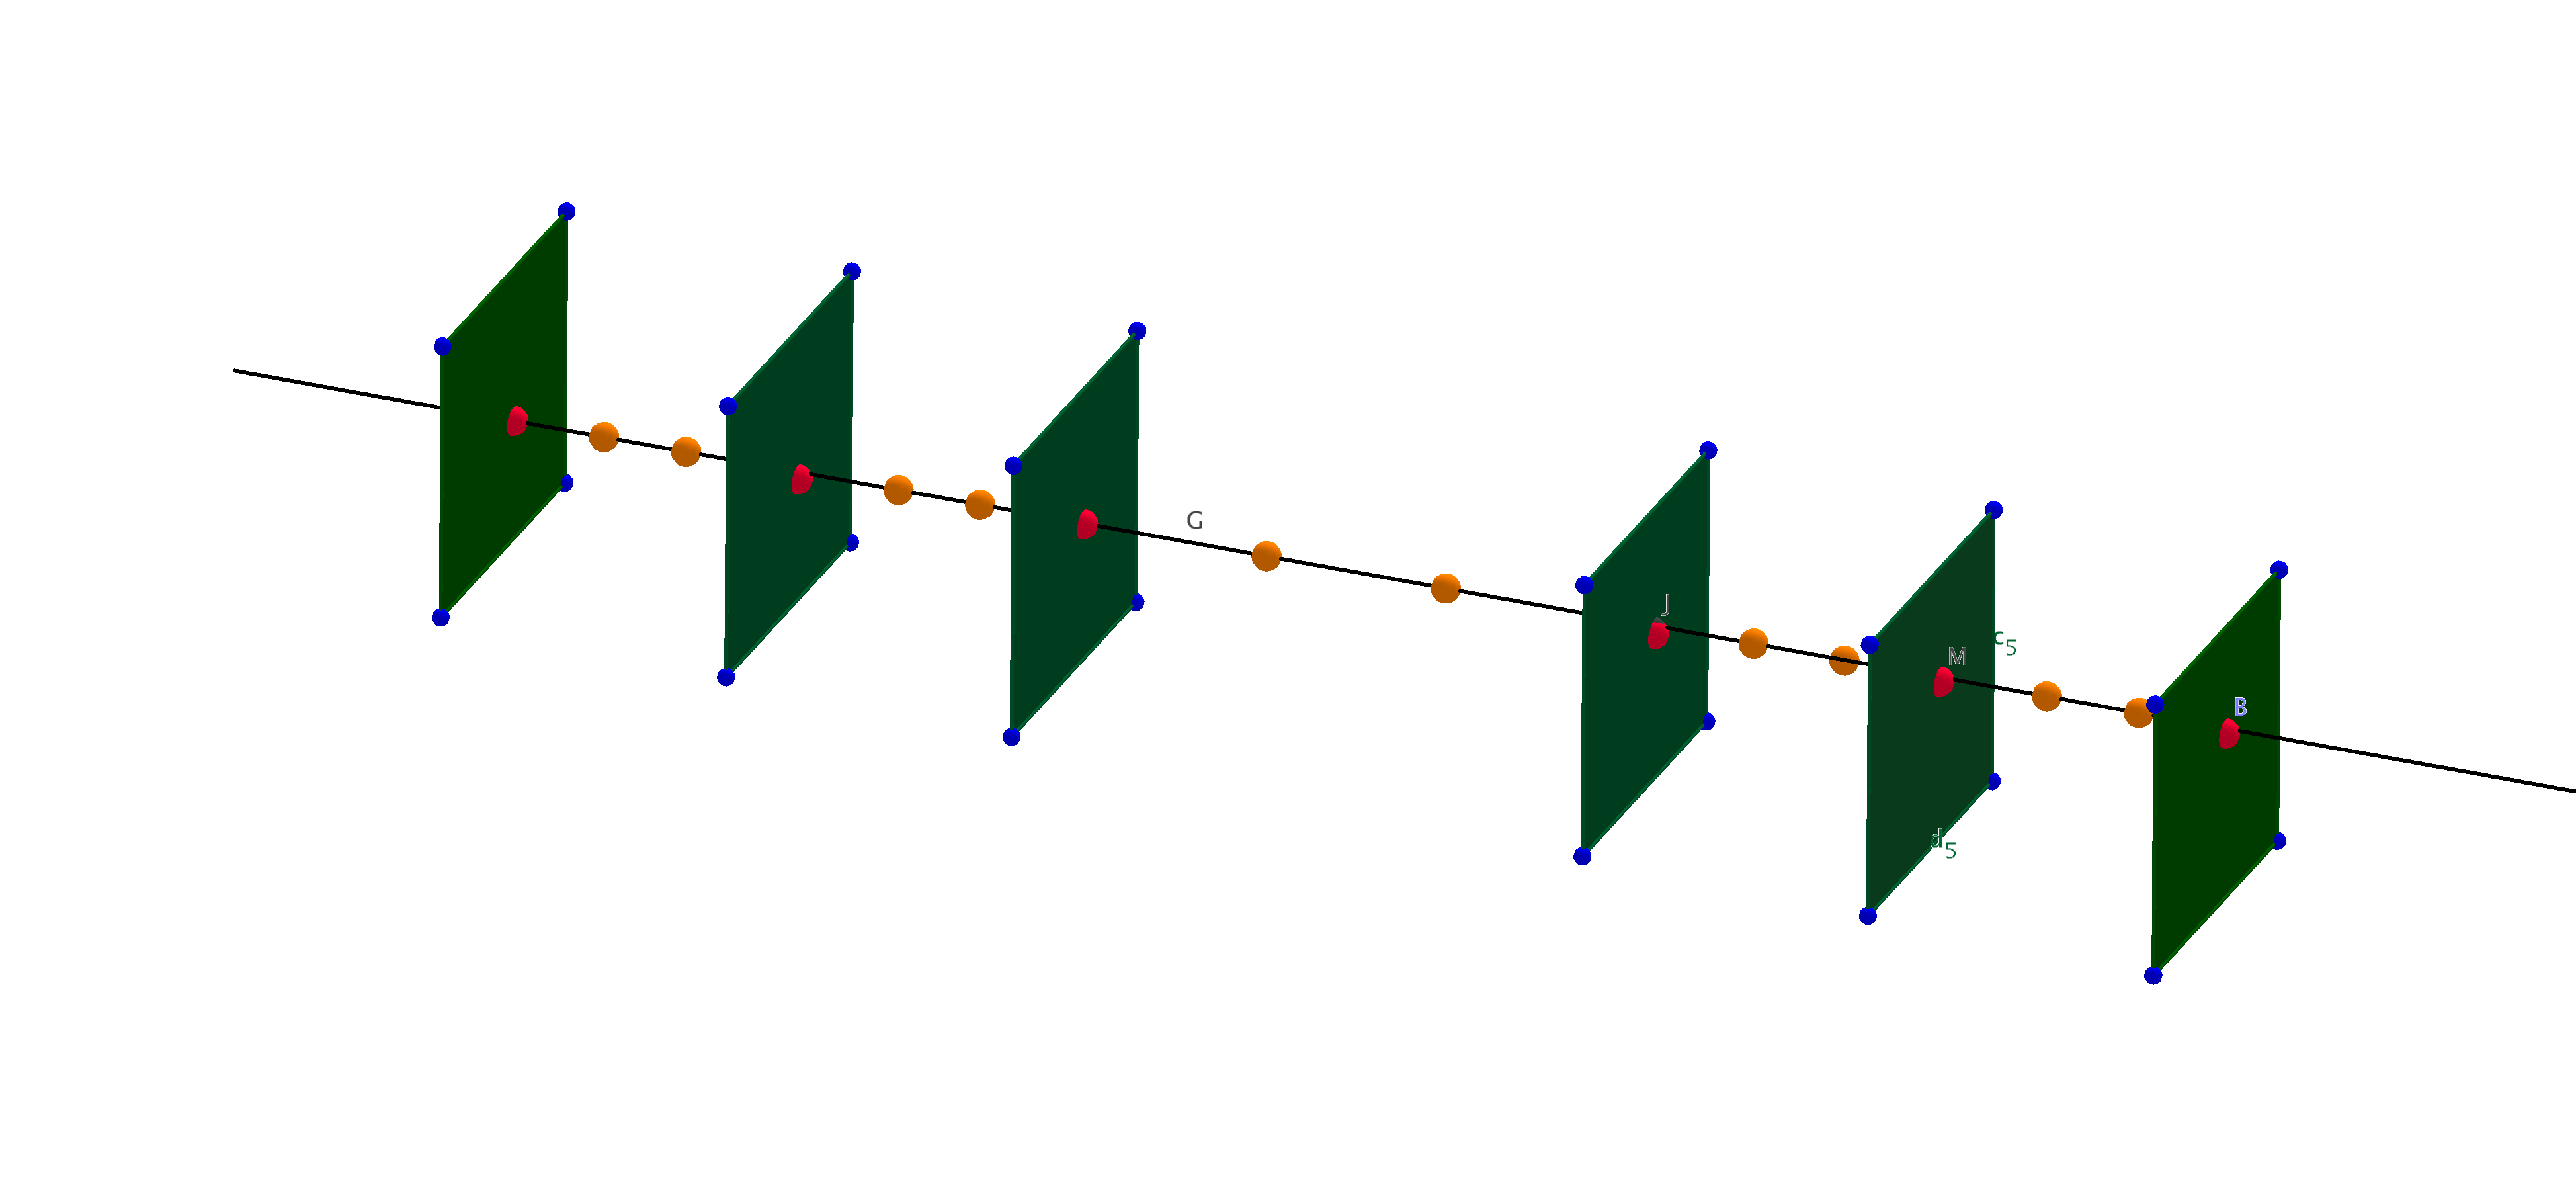
\includegraphics[scale=0.50]{pics/meas-scat-jac-link.png}
\caption{
\tiny{
\textcolor{red}{Red Dots: Measurements/Scattering} \textcolor{orange}{Orange Dots: Scattering}
}
}
\begin{itemize}
\item As many planes as you need can be added around the telescope.
\item Homogeneous sensors are modeled as thin scatterers
\item Inhomogeneous dead material between sensors modeled as two thin scatterers 
\end{itemize}

\end{figure}
\end{frame}

\begin{frame}
\frametitle{\textbf{2} Add Measurements}
\begin{figure}
\label{Meas}
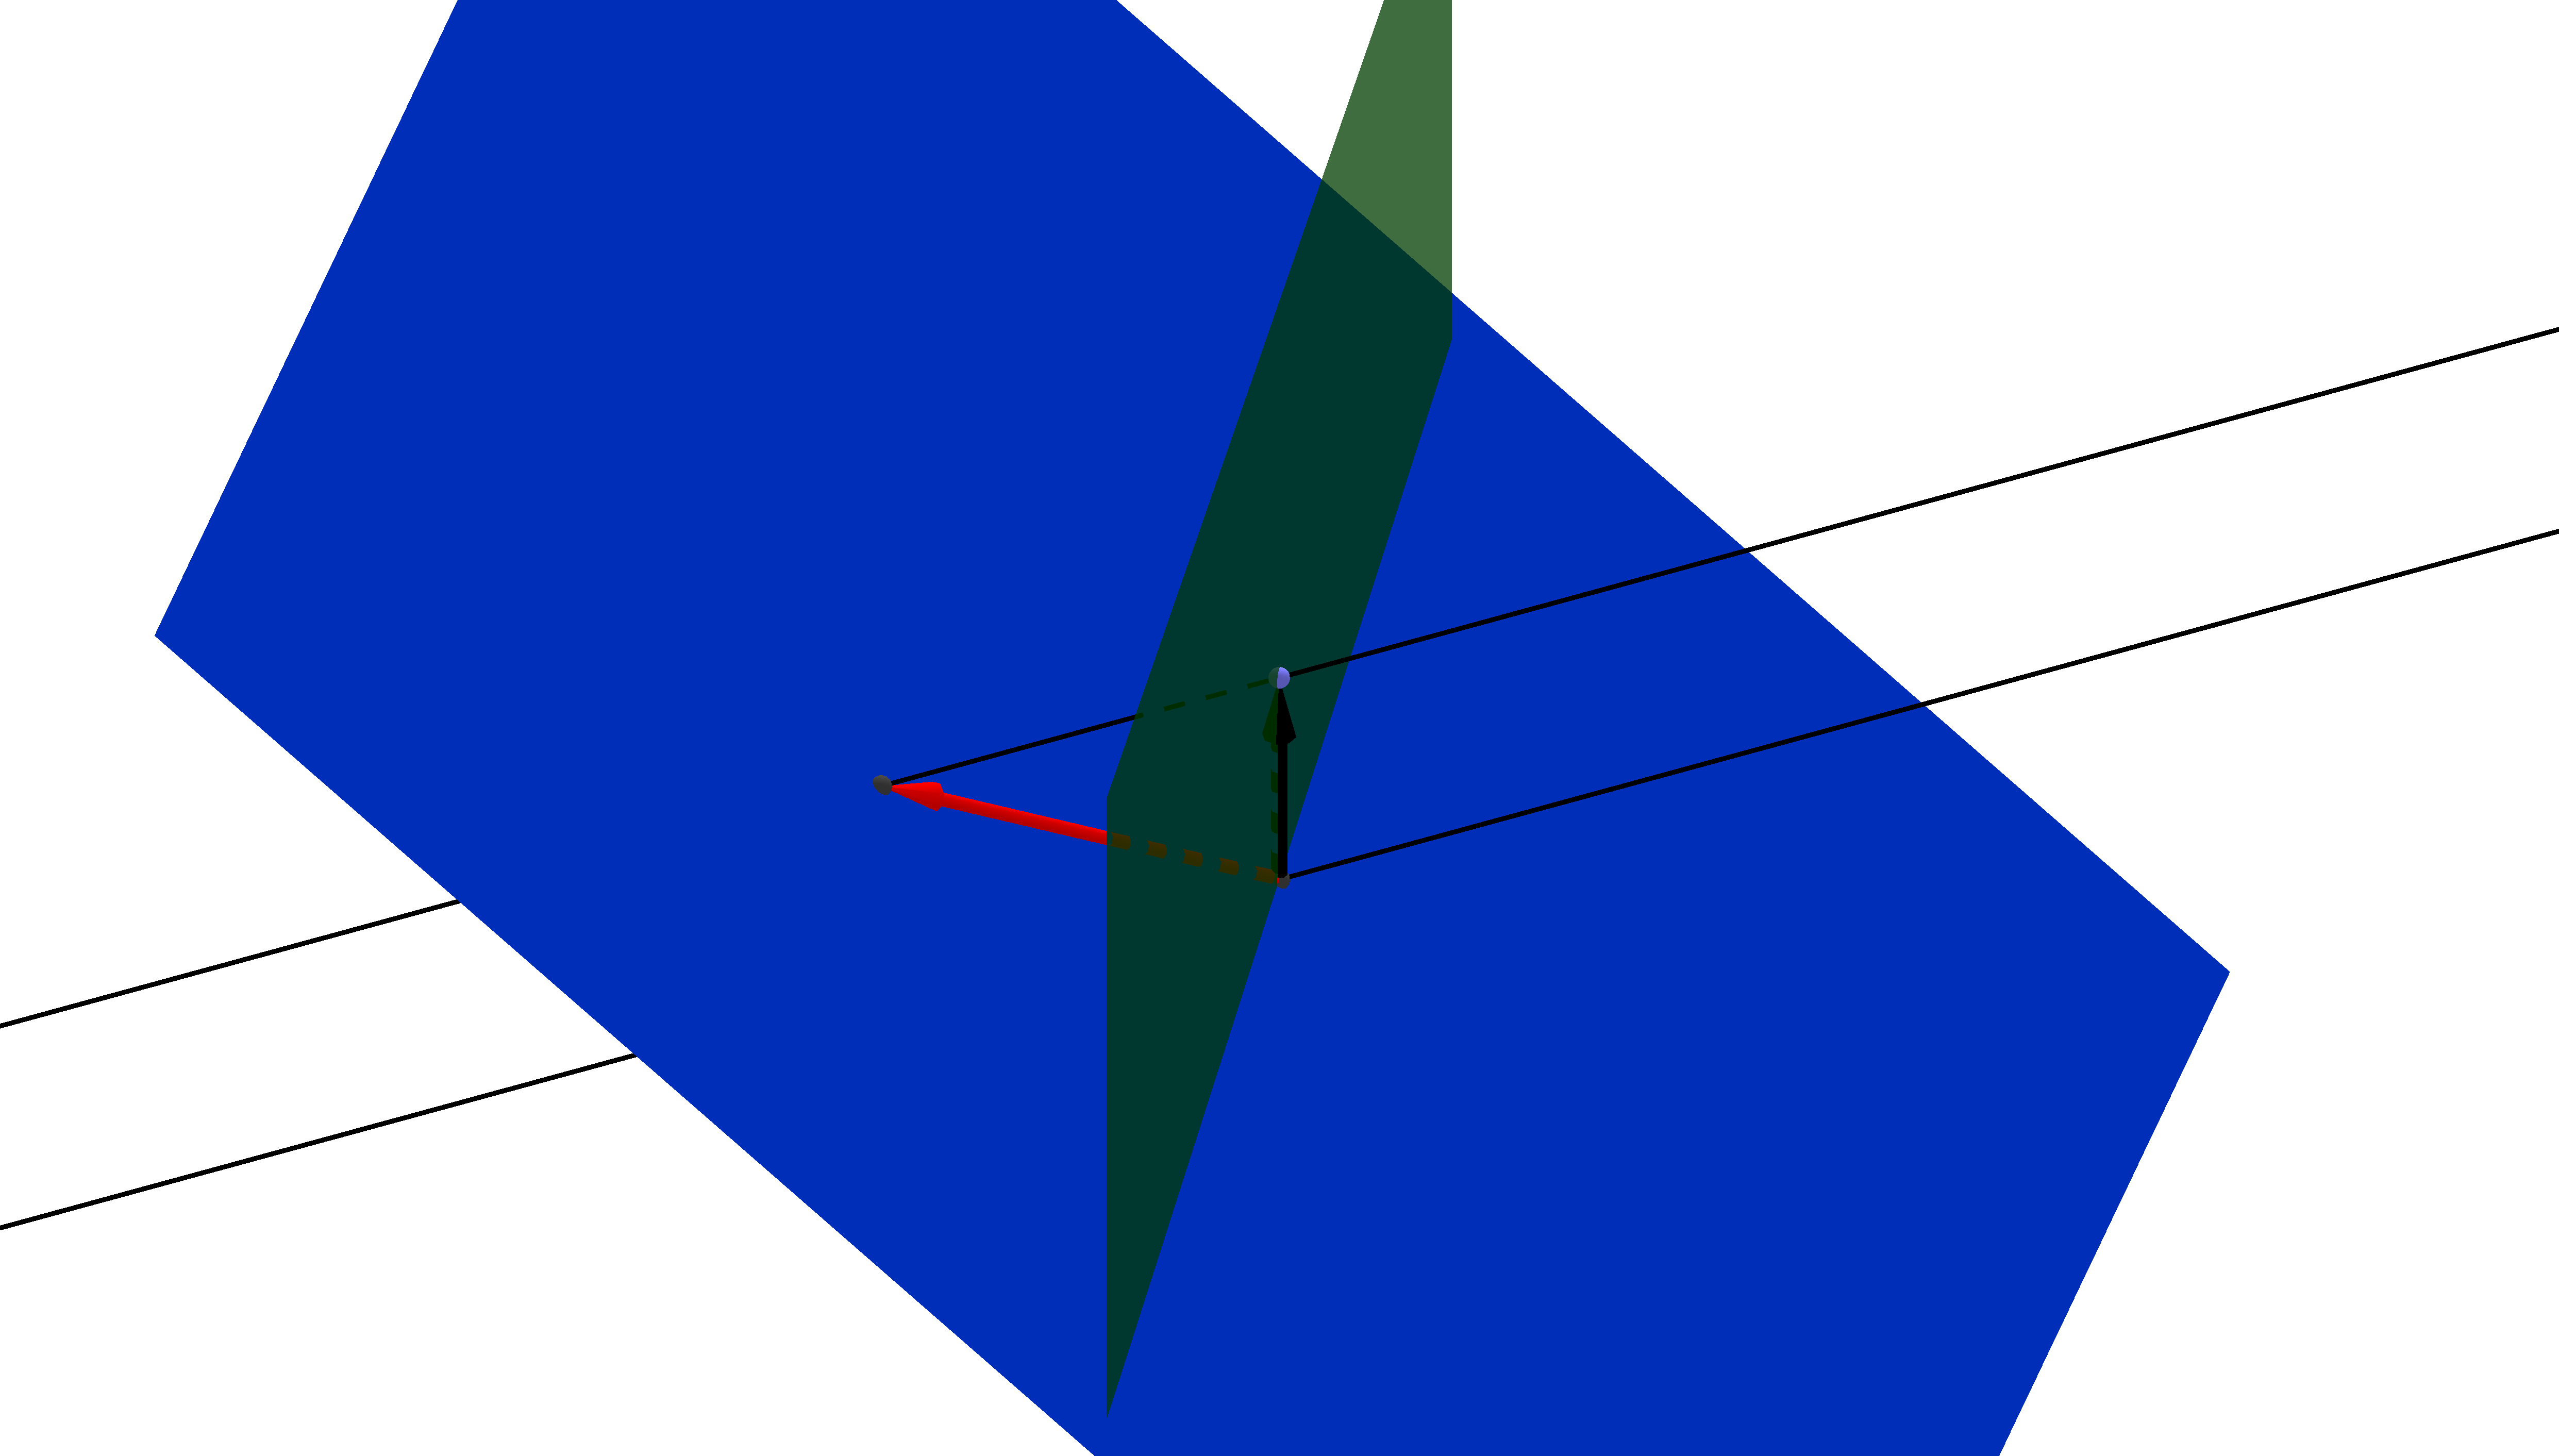
\includegraphics[width=0.5\linewidth]{pics/prop.png}
\caption{
\tiny{
\textcolor{green}{Green Plane: Local coordinate system XY plane (The sensor surface)}\newline
\textcolor{blue}{Blue Plane: Global Coordinate system which is shared by all sensors}\newline
\textcolor{black}{Black Lines: Track before/after motion}\newline
\textcolor{black}{Black Arrow: Change on track position in local frame}\newline
\textcolor{red}{Red Arrow: Change in track position in global frame}
} 
}
\begin{itemize}
\item Each plane has its own measurement frame.
\item Each hit contains all information needed to allow different locations on the sensor to have different measurement frames
\end{itemize}
\end{figure}
\end{frame}

\begin{frame}
\frametitle{\textbf{3} Add Scattering}
\begin{figure}
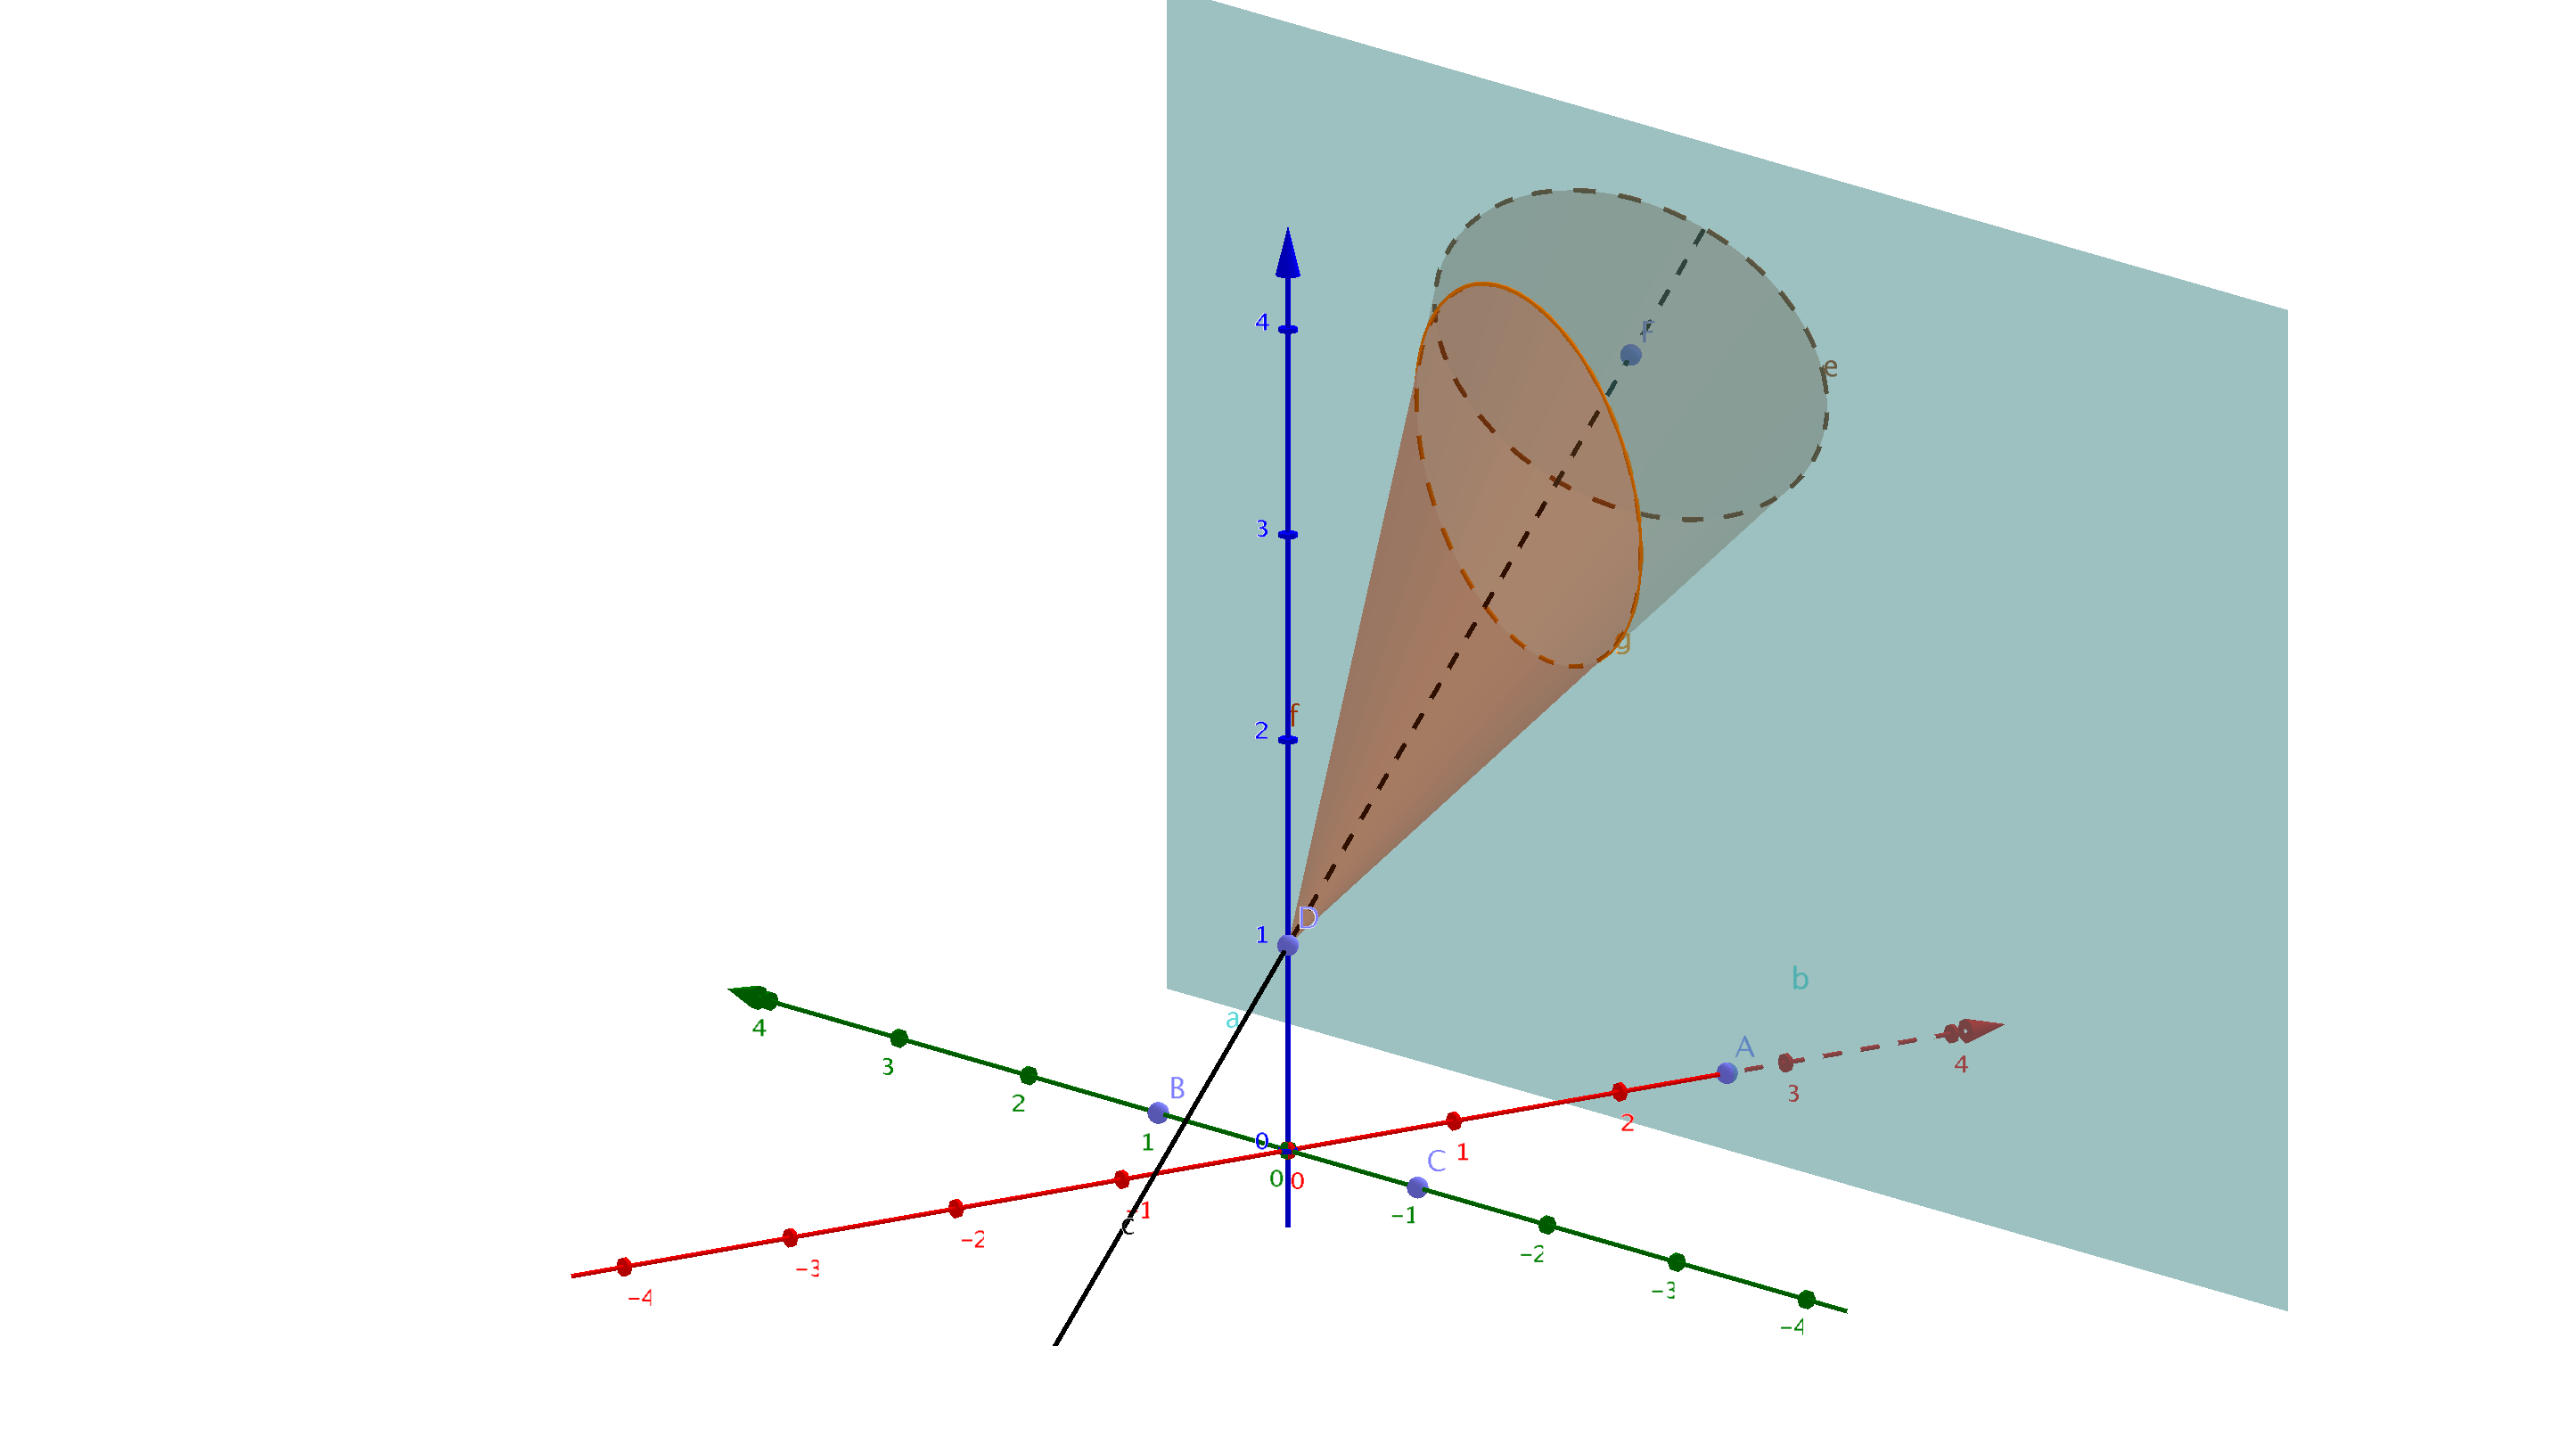
\includegraphics[width=0.65\linewidth]{pics/prop600GoodOffSensor.png}
\caption{\tiny{
\textcolor{black}{Black Line: Track}  \textcolor{orange}{Orange Cone: The position errors due to a thin scatterer} \textcolor{blue}{Blue Plane: Measurement plane.} \newline
}
}
\label{fig:ScatFrame}
\begin{itemize}
\item Kink angles are included in fit rather than placed as addition uncertainty. 
\item A simple or complex determination of the radiation length with the particles path can be used.
\end{itemize}
\end{figure}
\end{frame}

\begin{frame}
\frametitle{\textbf{4} Alignment}
\begin{figure}
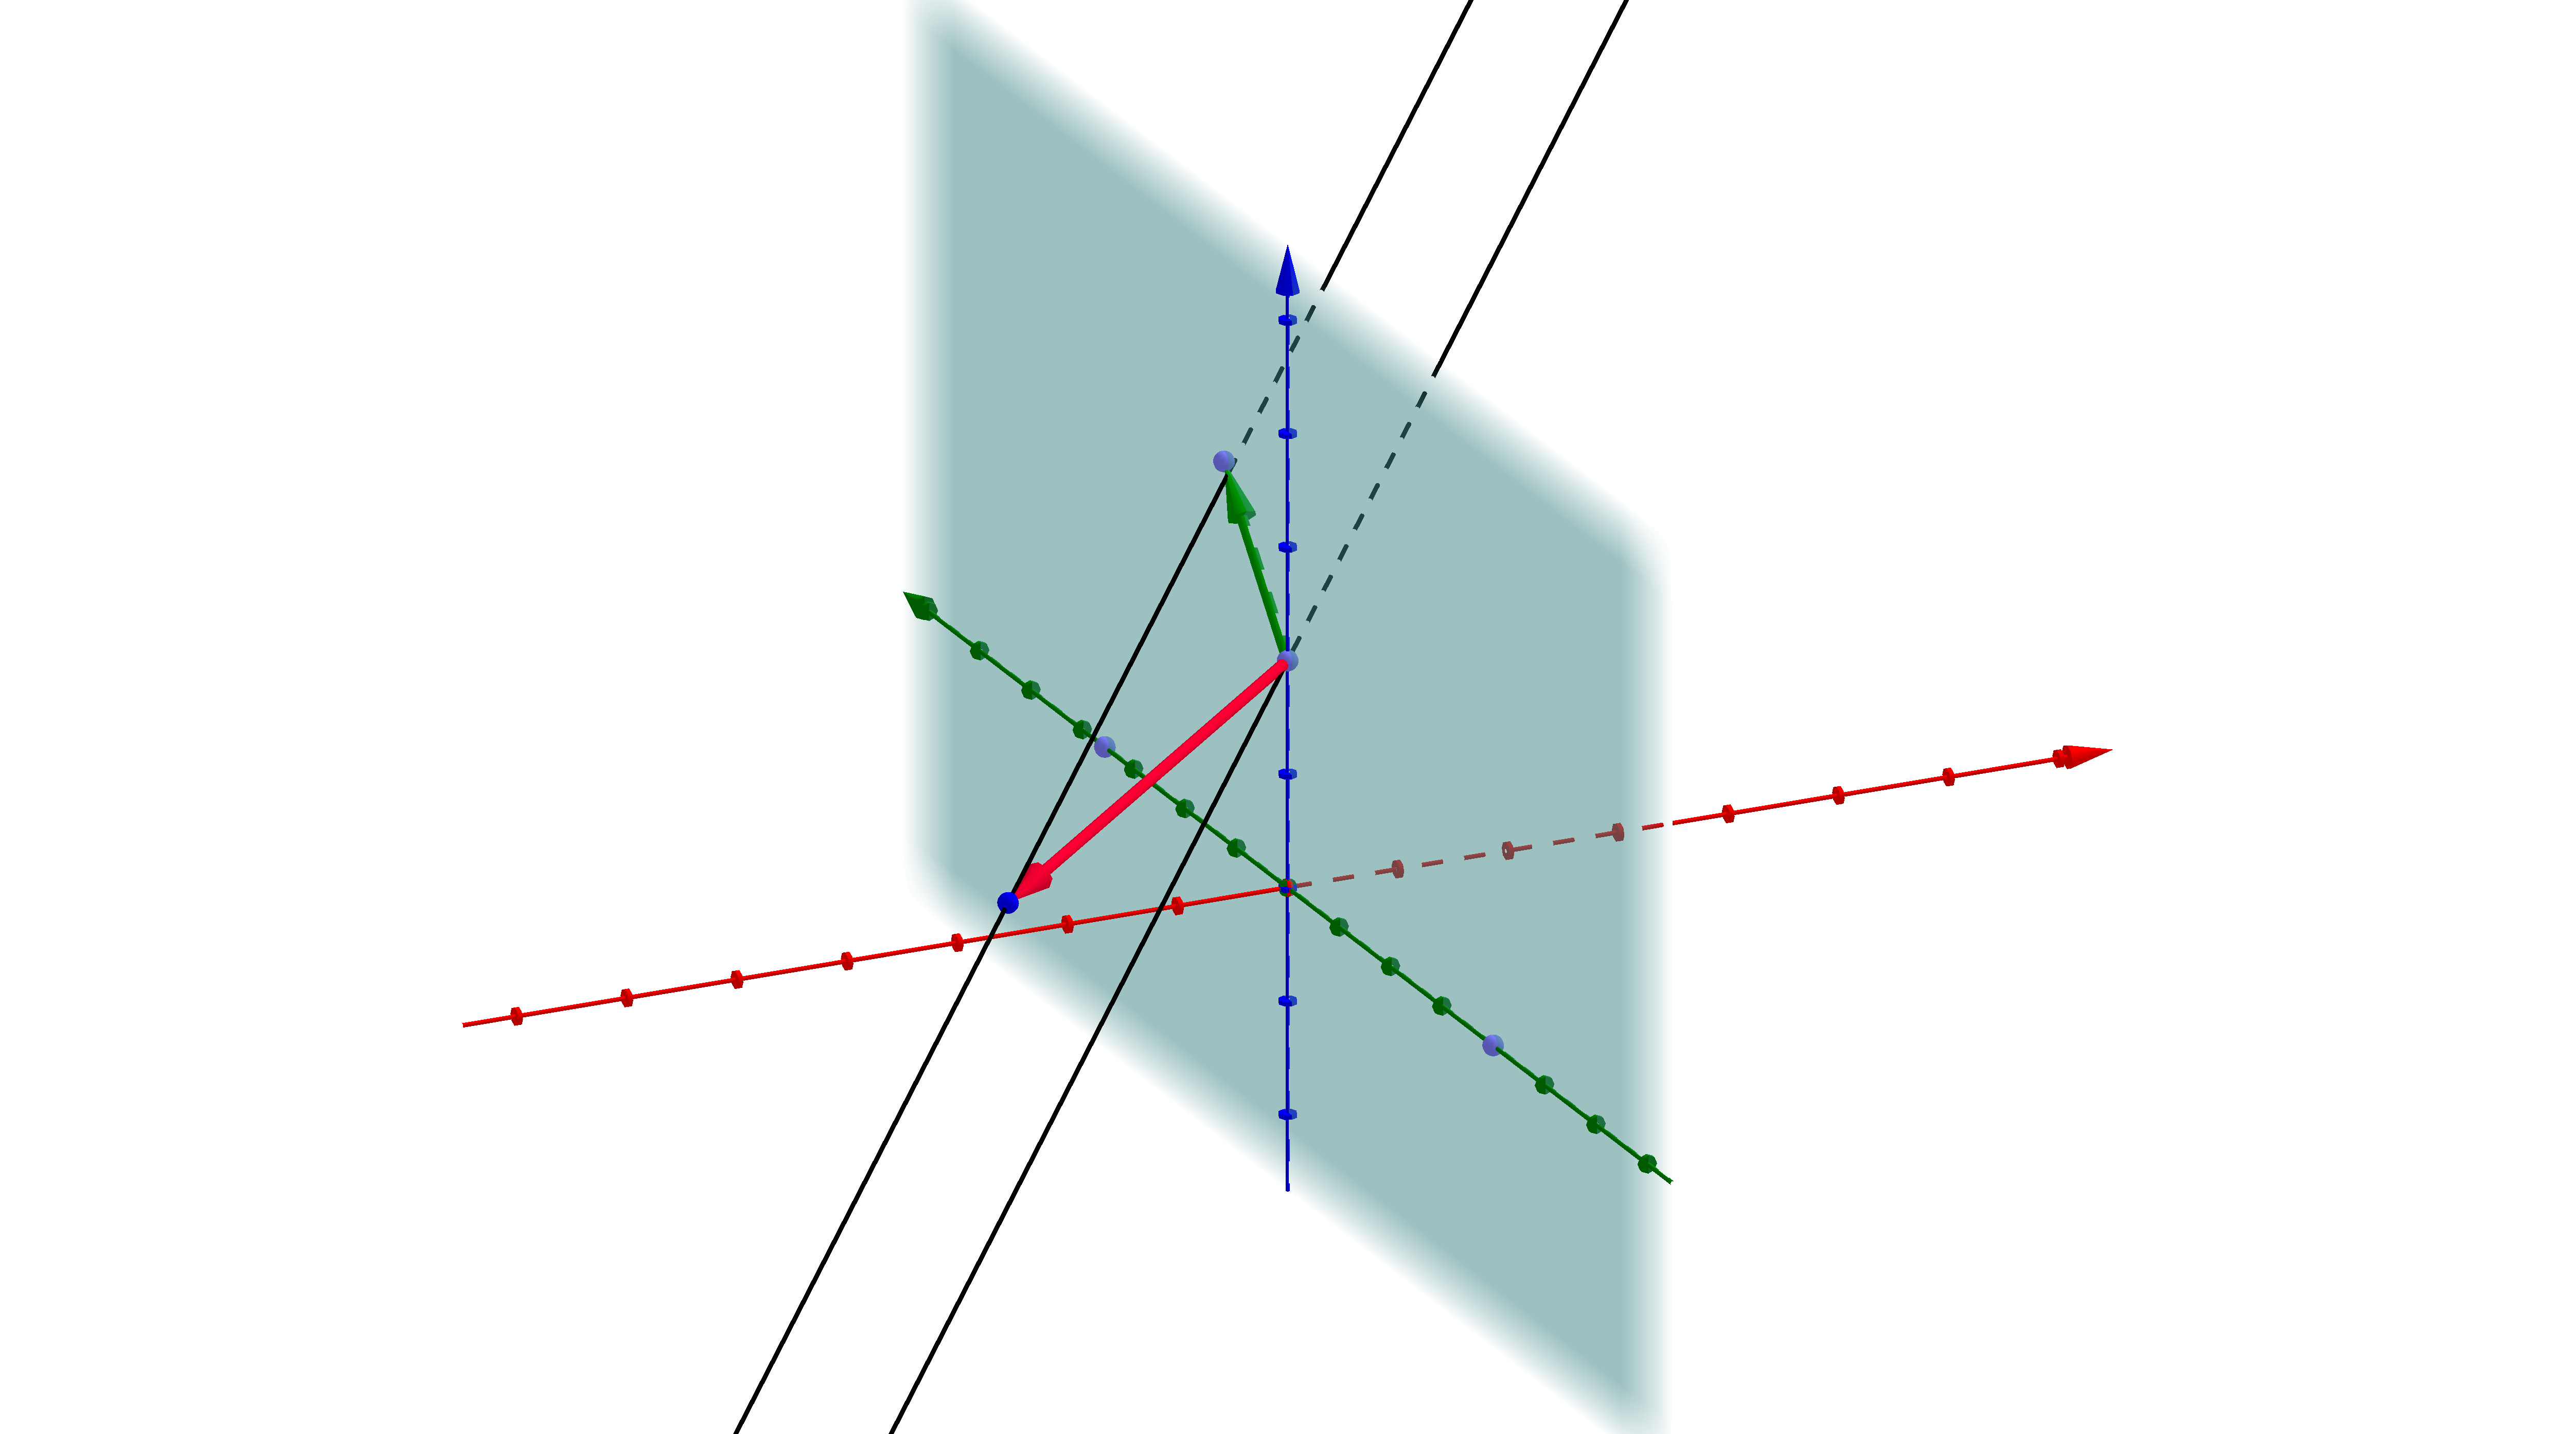
\includegraphics[width=0.6\linewidth]{pics/alignBigger.png}
\caption{\tiny{
\textcolor{black}{Black Line: Track} \newline
\textcolor{red}{Red Arrow: The change in location of track due to change in coordinate system of sensor}\newline
\textcolor{green}{Green Arrow: Change on sensor surface in global frame. } 
}
}
\begin{itemize}
\item All track variables are included as local (nuisance) parameters. 
\item Geometry information is updated and stored in a single location.
\item Final track fitting results are output in ROOT/LCIO format.
\item Analysis and selection code exists
\end{itemize}
\label{fig:TC1}
\end{figure}
\end{frame}

\section{Examples and Results}
\subsection{A Quick Comparison of DAF and GBL}
\begin{frame}
\frametitle{A Quick Comparison of DAF and GBL}
\begin{columns}[t]
\column{0.5\textwidth}
\centering
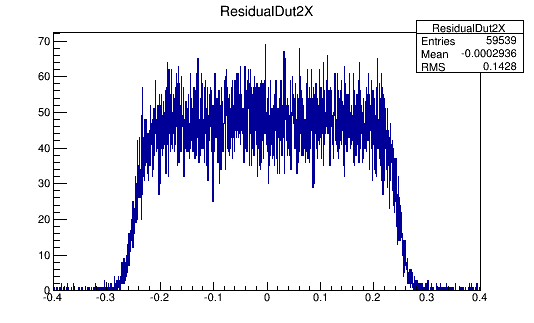
\includegraphics[width=0.8\linewidth]{pics/DataDESYNov13_GBL_DUT21_ResidualX.png}\\
\tiny{\textbf{GBL X residual}}\\
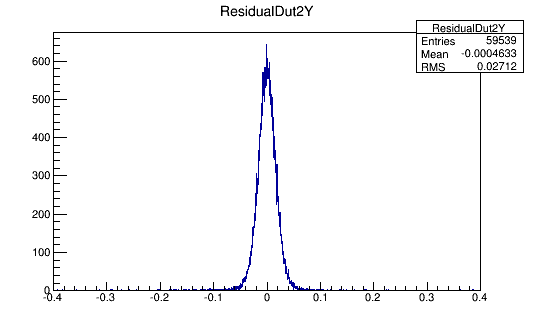
\includegraphics[width=0.8\linewidth]{pics/DataDESYNov13_GBL_DUT21_ResidualY.png}\\
\tiny{\textbf{GBL Y residual}}\\
\column{0.5\textwidth}
\centering
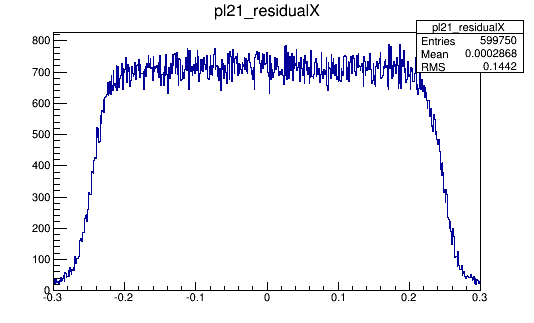
\includegraphics[width=0.8\linewidth]{pics/DESYNOV13_DUT21_ResidualX.png}\\ 
\tiny{\textbf{DAF X residual}} \\
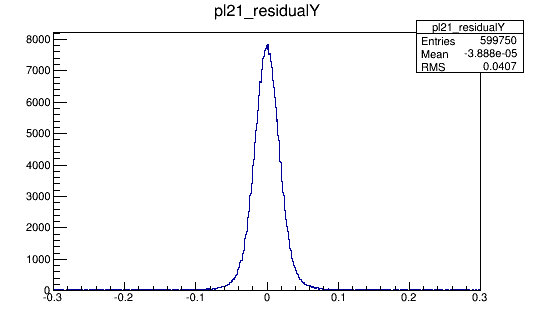
\includegraphics[width=0.8\linewidth]{pics/DESYNOV13_DUT21_ResidualY.png}\\ 
\tiny{\textbf{DAF Y residual}} \\
\end{columns}
\tiny{Plots: Ryan Nelson}
\vspace{5pt}
\end{frame}
\subsection{Example Output from Quad Module}
\begin{frame}
\frametitle{Example Output from the Quad Module}
\begin{columns}[t]
\column{0.5\textwidth}
\centering
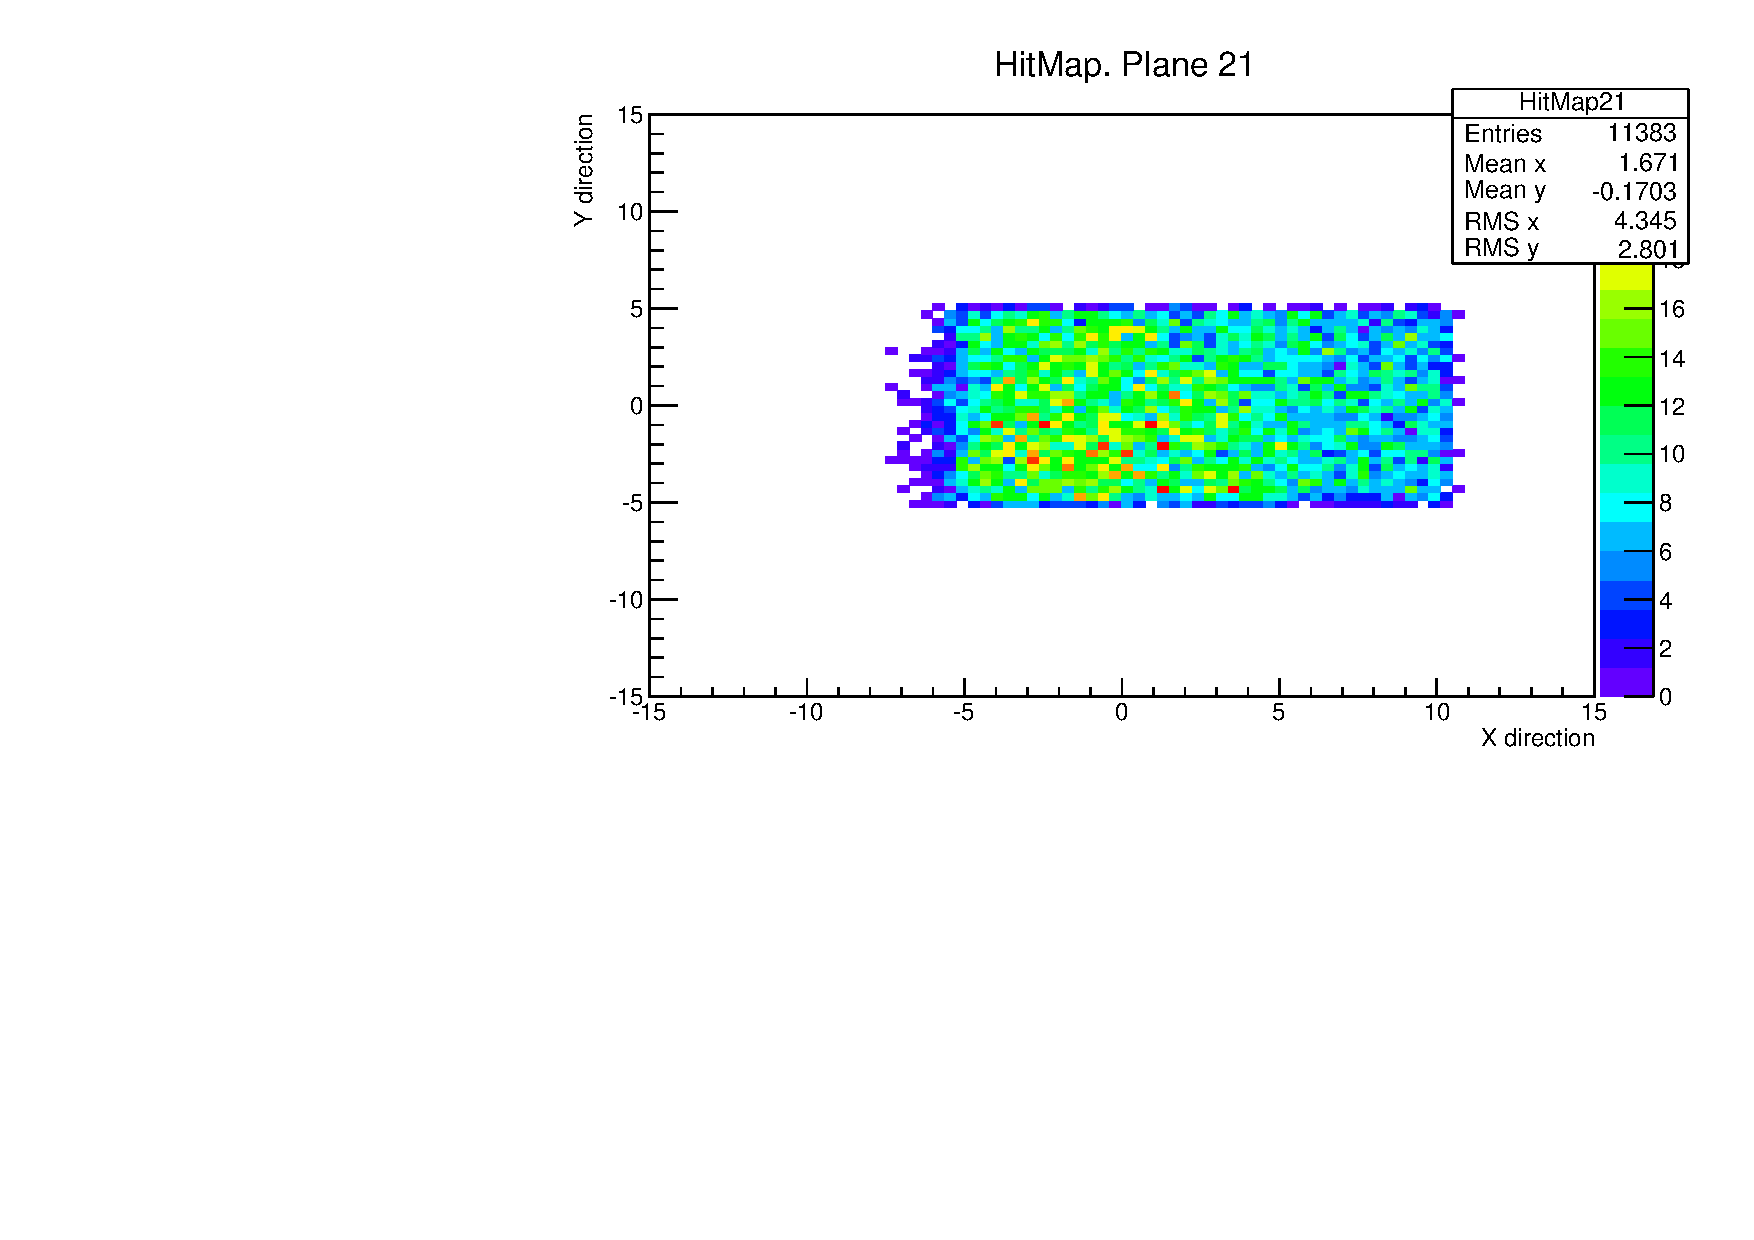
\includegraphics[width=0.8\linewidth]{pics/HitMapQuadAfterTrack.pdf}\\
\tiny{\textbf{Hit map after tracking in local frame \\
(Beam spot can be seen here)}}\\
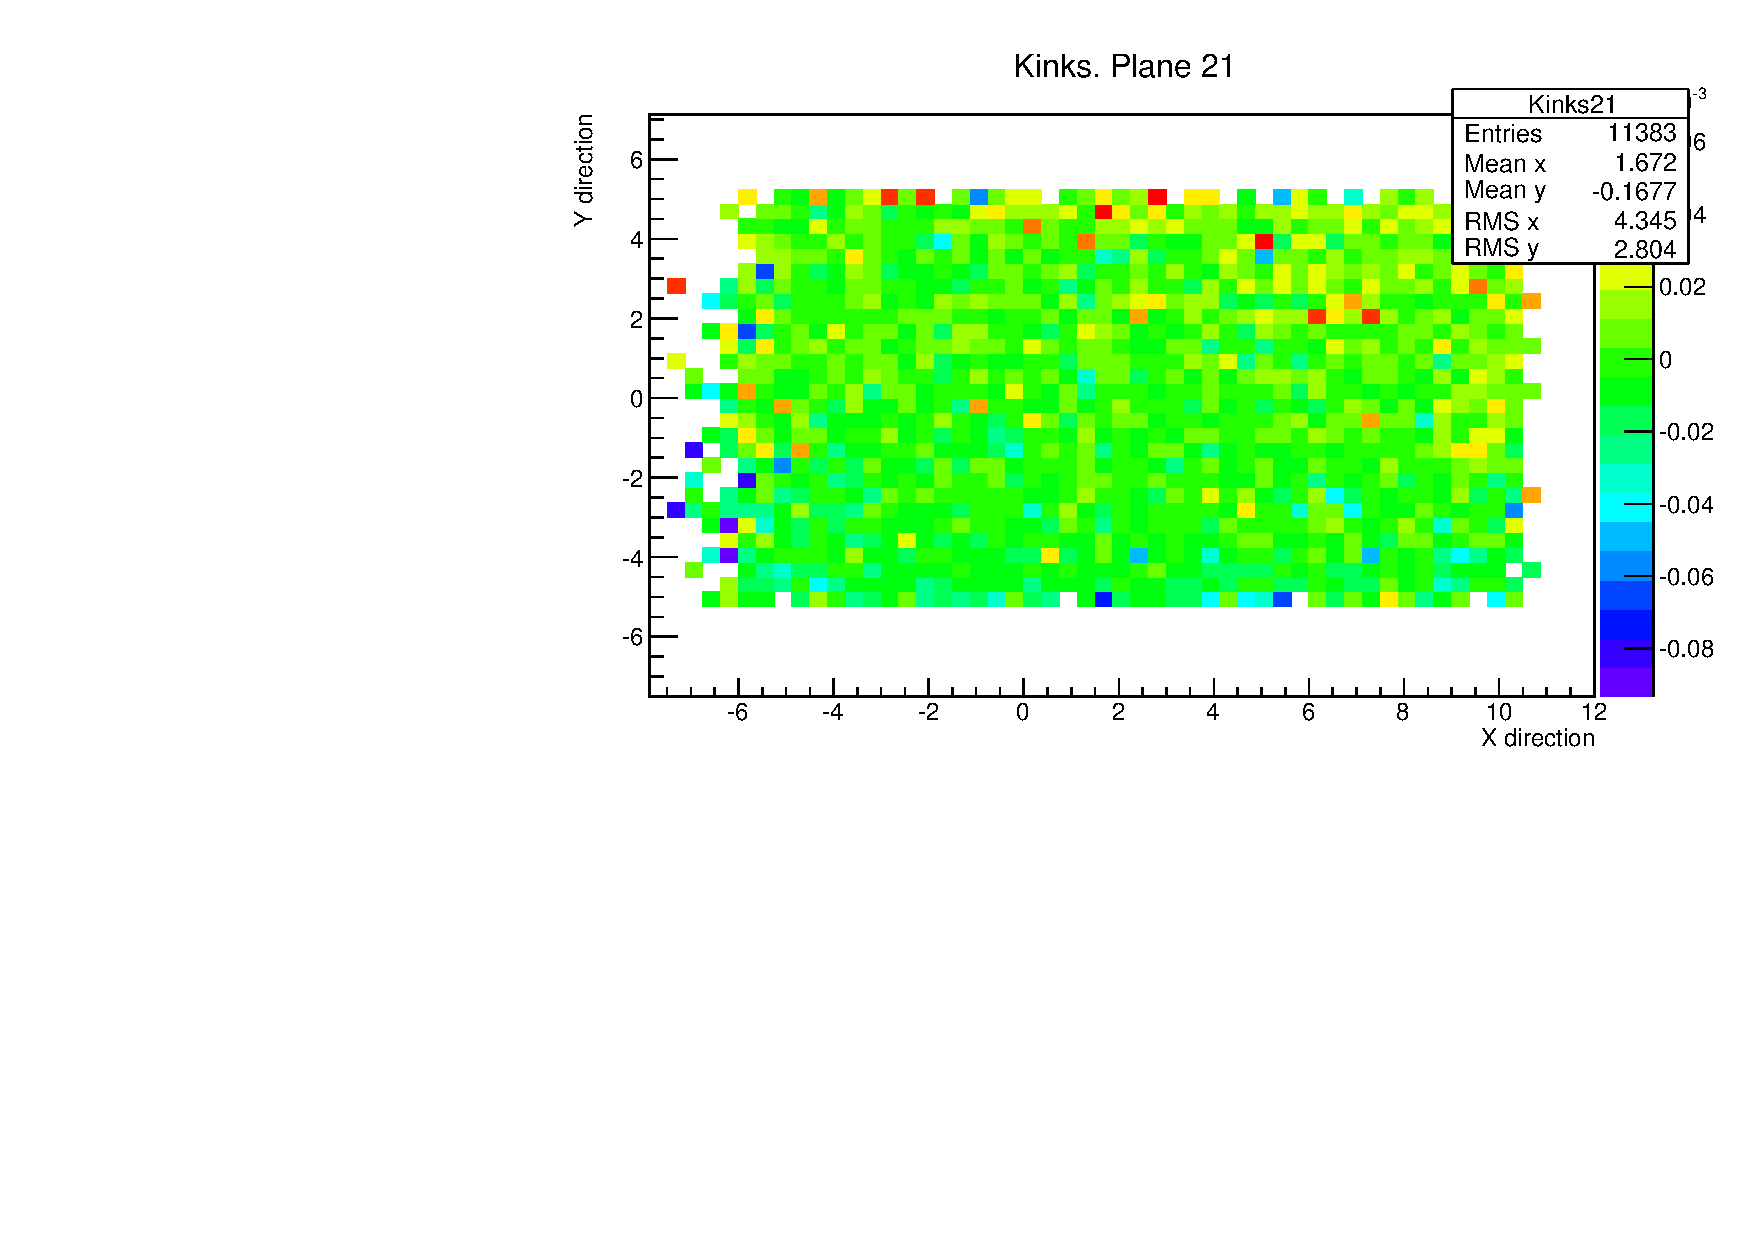
\includegraphics[width=0.8\linewidth]{pics/kinksQuad.pdf}\\
\tiny{\textbf{Kinks in local frame\\
 (Expect to be zero since scattering is random process about the initial incidence)}}\\
\column{0.5\textwidth}
\centering
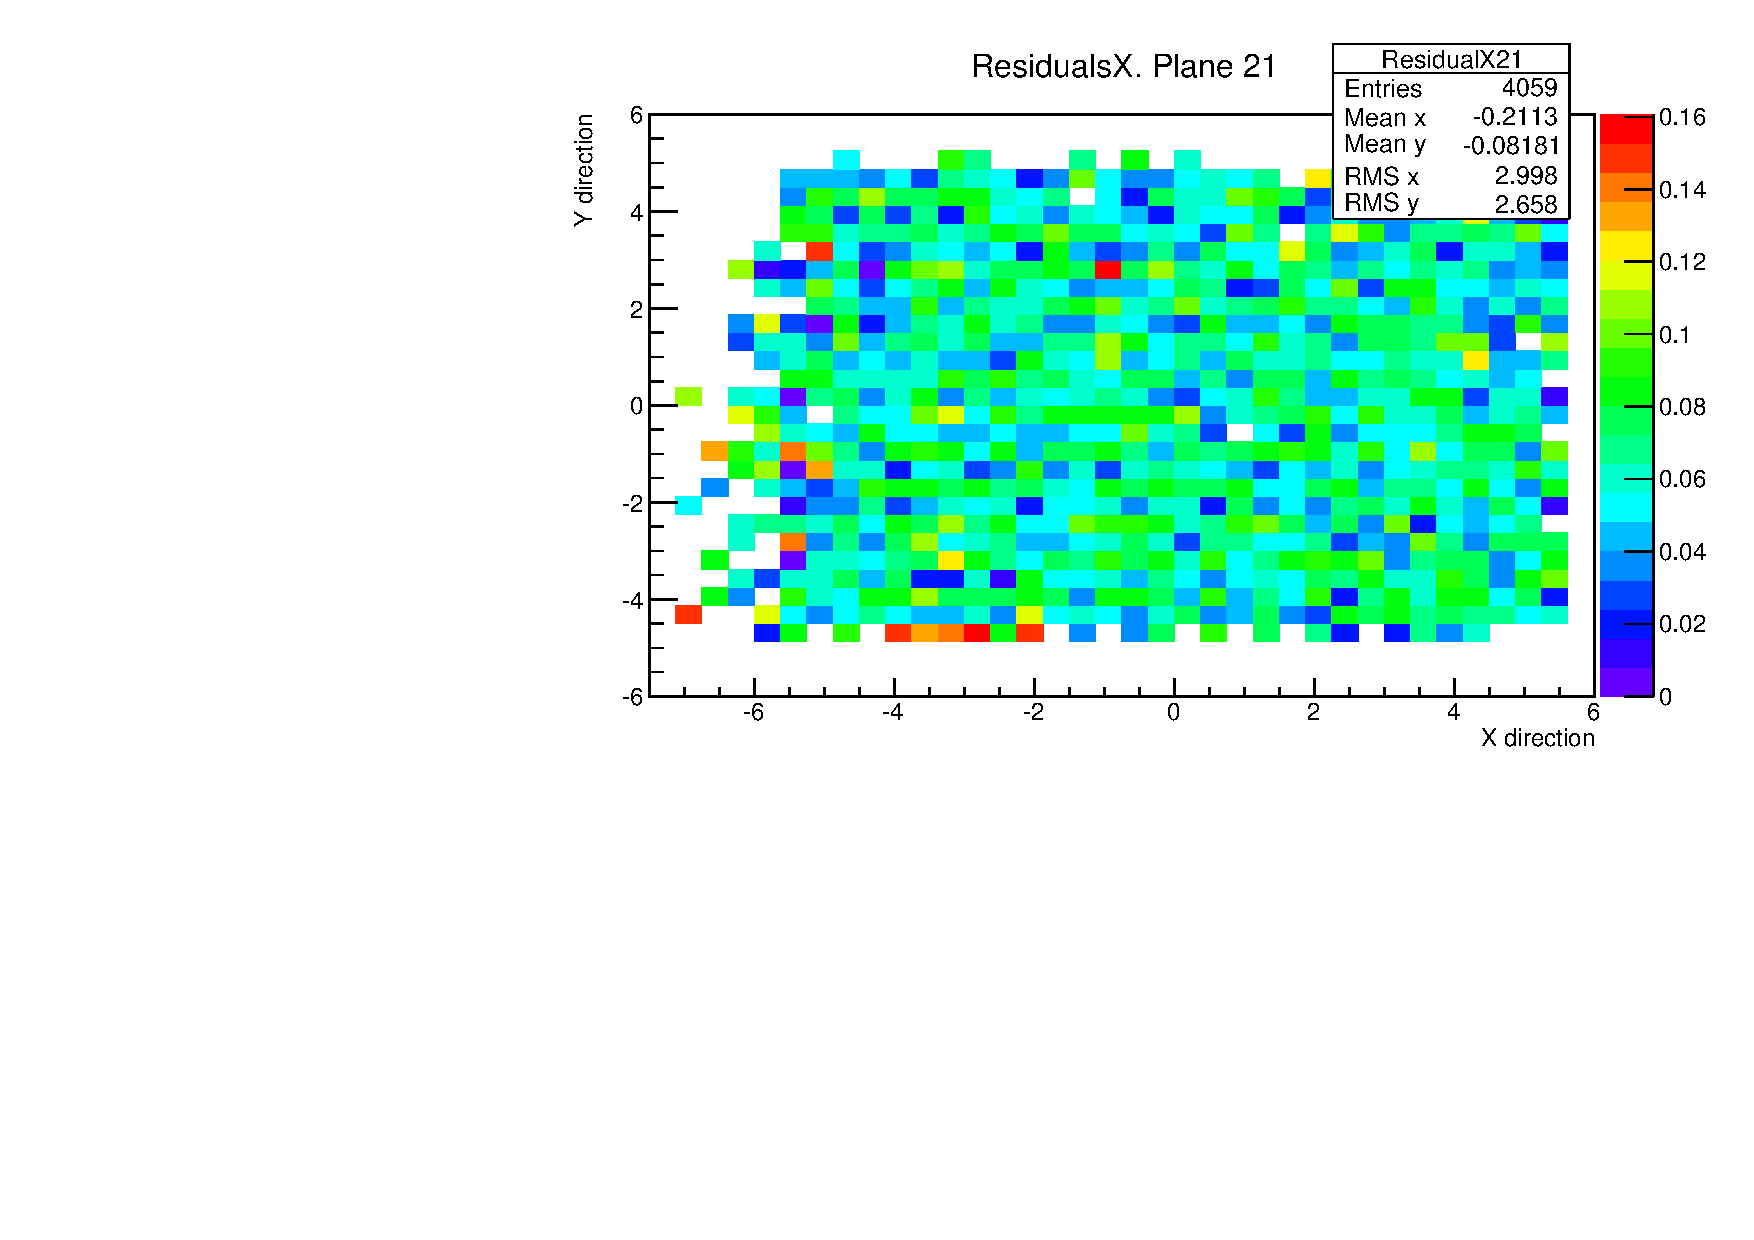
\includegraphics[width=0.8\linewidth]{pics/QuadXRes73Micron.pdf}\\ 
\tiny{\textbf{Residual on surface of sensor in local X direction \\
 ($\sim$70 \si{\micro\metre} intrinsic resolution)}}

\tiny{
\vspace{10pt}
Quad modules are large area pixel sensors mounted on 4 FEI4 readout ASICs \\
\vspace{10pt}
Results look as expected for 250x50 $\si{\micro\metre\squared}$ sensor assuming uniform distribution on each pixel. \\
\vspace{10pt}
Efficiency measurements will be performed on these modules with particular interest in the long/ganged pixel regions. \\
\vspace{10pt}
Track/State/Hit/Cluster objects are arranged in a simple hierarchy to allow easy additions to code.\\
}
\end{columns}
\end{frame}

\begin{frame}
\frametitle{Efficiency Measurements}
\begin{columns}[t]
\column{0.5\textwidth}
\centering
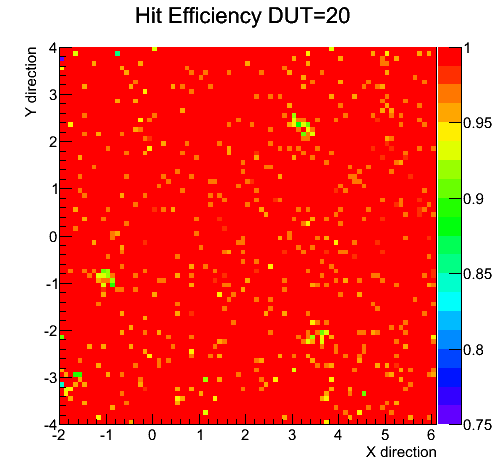
\includegraphics[width=0.65\linewidth]{pics/desy250x50AC_250x50DC_20V20.png}\\
\tiny{\textbf{AC Sensor biased 20V }}\\
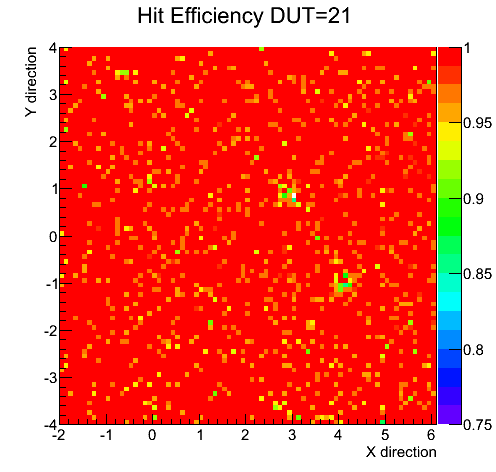
\includegraphics[width=0.65\linewidth]{pics/desy250x50AC_250x50DC_20V21.png}\\
\tiny{\textbf{DC Sensor biased 20V}}\\
\column{0.5\textwidth}
\centering
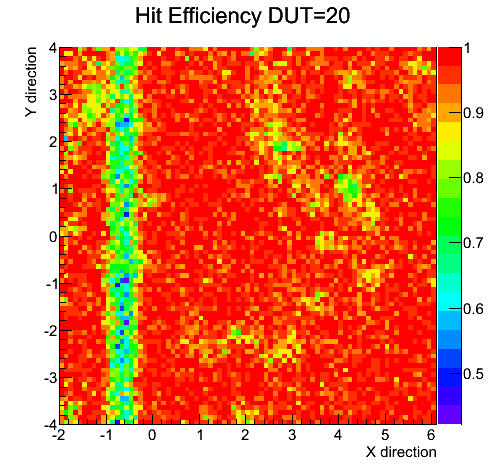
\includegraphics[width=0.65\linewidth]{pics/desy250x50irad_250x50DC_200V20.png}\\ 
\tiny{\textbf{AC Sensor irradiated to $10^{15}$ $n_{eq} cm^{-2}$ biased 200V.}}

\tiny{
\vspace{10pt}
 In effort toward the ATLAS upgrade, efficiency measurements have been performed on different sensors irradiated to different fluencies at the DESY testbeam. \\ 
\vspace{10pt}
Pitch 250x50 \si{\micro\metre\squared} with different coupling.\\
\vspace{10pt}
DC and AC sensor shows comparable efficiencies.\\
\vspace{10pt}
Radiation damage is clearly visible for irradiated sensor.\\
\vspace{10pt}
Plots: Helen Hayward.
}
\end{columns}
\end{frame}

\subsection{Efficiency Measurements with ATLAS12 Strip Sensor}
\begin{frame}
\frametitle{Efficiency Measurements with ATLAS12 Strip Sensor}
\begin{columns}[t]
\column{0.5\textwidth}
\centering
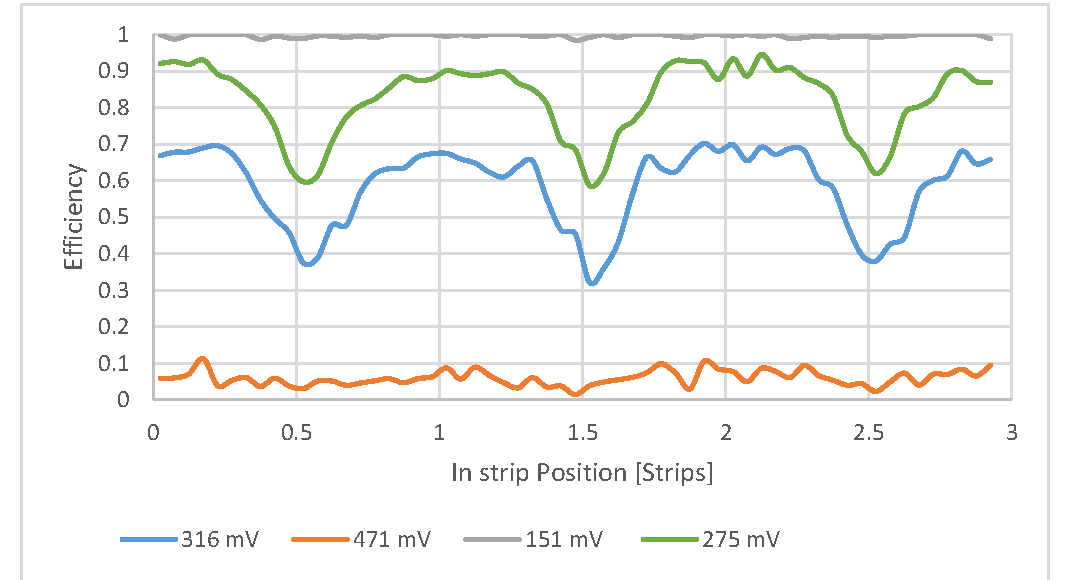
\includegraphics[width=0.9\linewidth]{pics/may2015Testbeam_cropped.pdf}\\
\tiny{\textbf{Combined efficiency for each strip with different thresholds}}\\
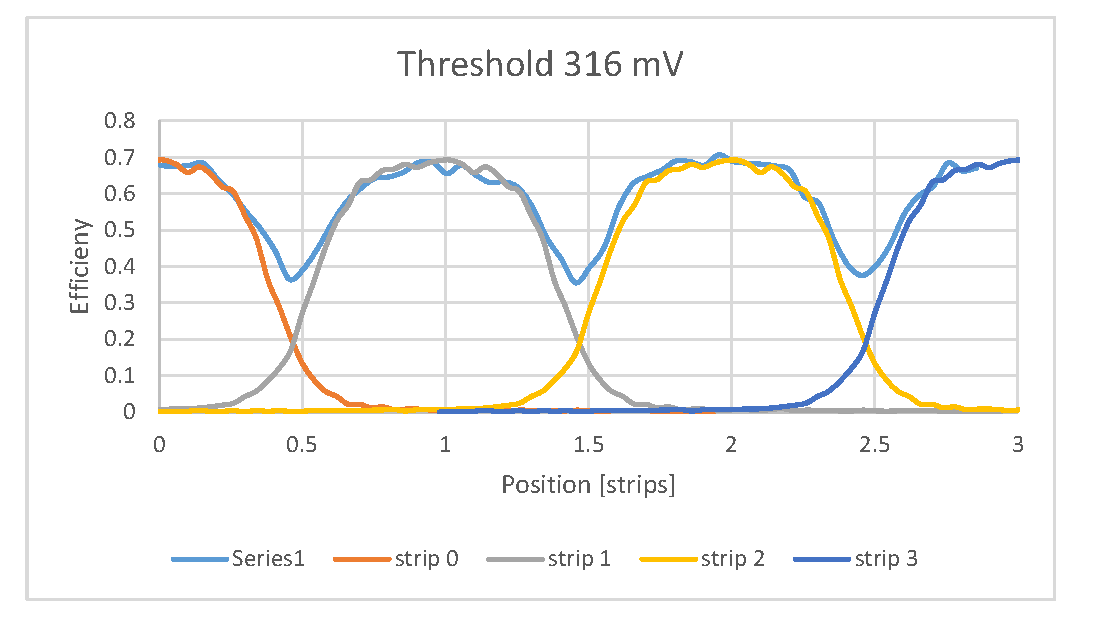
\includegraphics[width=0.9\linewidth]{pics/eff_strip.pdf}\\
\tiny{\textbf{Combined efficiency for each strip for 316 mV  threshold. }}\\
\column{0.5\textwidth}
\centering
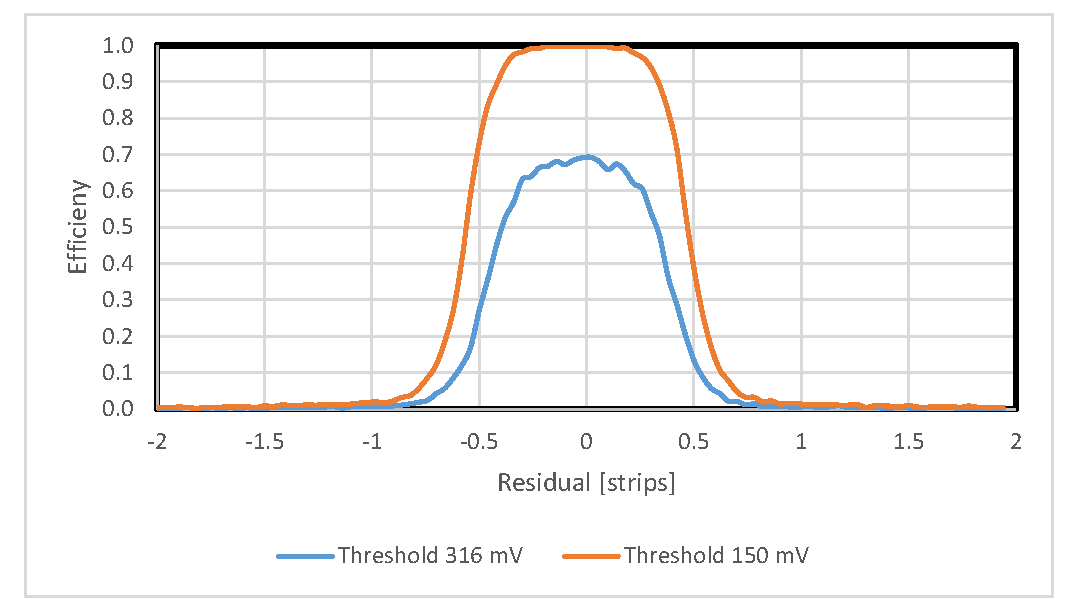
\includegraphics[width=0.9\linewidth]{pics/eff_strip_single_cropped.pdf}\\ 
\tiny{\textbf{Efficiency with distance from centre of strip.}}

\tiny{
\vspace{10pt}
ATLAS12 Strip Sensor (74.5 \si{\micro\metre\squared} pitch). \\
\vspace{10pt}
Interested in individual strips efficiency. Requires accurate prediction on DUT.\\
\vspace{10pt}
Using analysis code which is part of the SCT example.\\
\vspace{10pt}
Plots: Richard Peschke.
}
\end{columns}
\end{frame}

\section{Conclusion}
\begin{frame}
\frametitle{Conclusion}
A generic track fitting model has been implemented into EUTelecope.
\begin{itemize}
\item Many working examples which can be used as the bases for future work.
\item Designed to work for the widest range of testbeam setups.
\item Output comes in a range of formats for different analysis tools and packages. 
\end{itemize}
Future additions
\begin{itemize}
\item Radial strips and improvement in the implementation of the measurement frame.
\item Replacing the old GEAR file format to allow more complex geometries.
\end{itemize}
\end{frame}

\begin{frame}
Backup
\end{frame}
\section{Additional Information}
\subsection{Magnetic Fields}
\begin{frame}
\frametitle{Magnetic Fields}
\begin{figure}
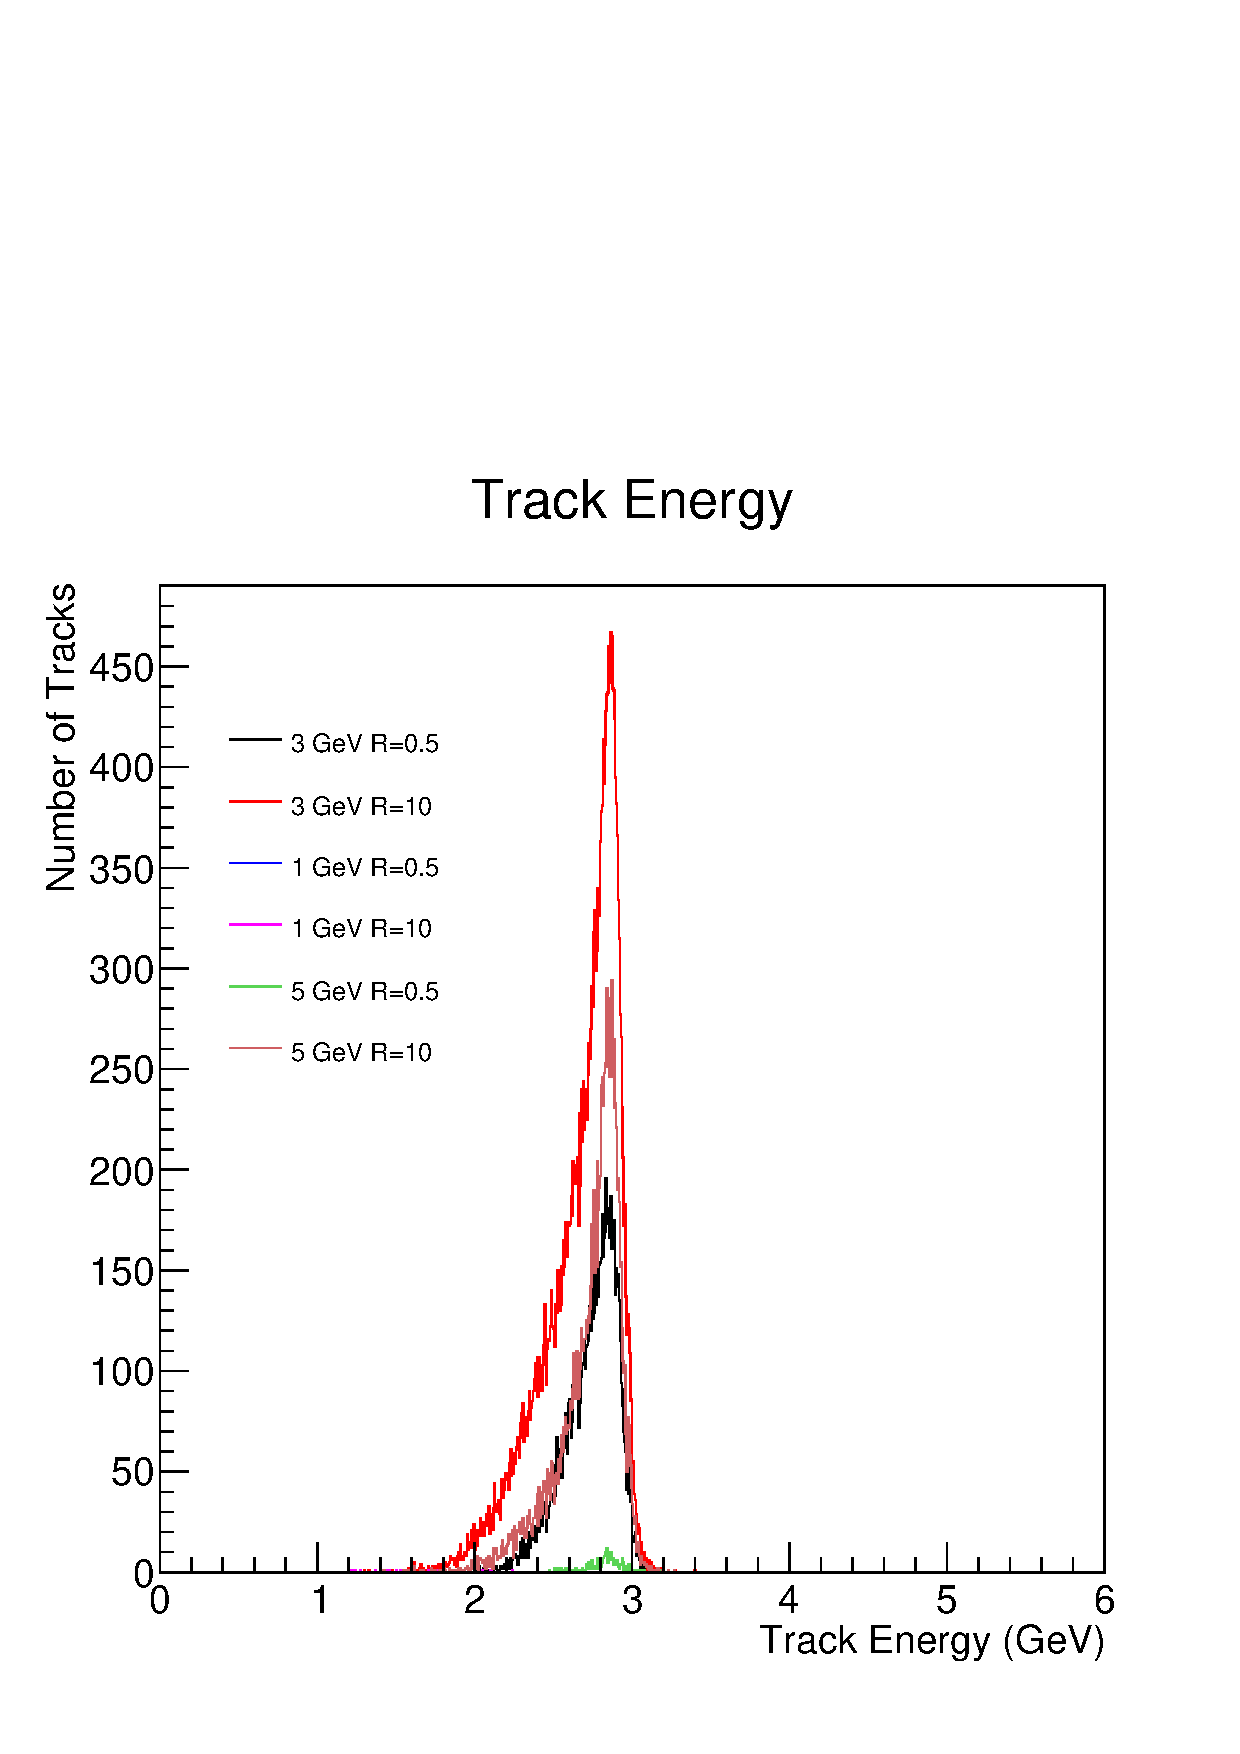
\includegraphics[width=0.45\linewidth]{pics/beamE3B1.pdf}
\tiny{
\caption{Different pattern recognition inputs to check the consistency of the track fitting}
}
\end{figure}
\end{frame}

\subsection{Current Testbeam Reconstruction}
\begin{frame}
\frametitle{Current Testbeam Reconstruction (October 2015)}
\begin{columns}[t]
\column{0.5\textwidth}
\centering
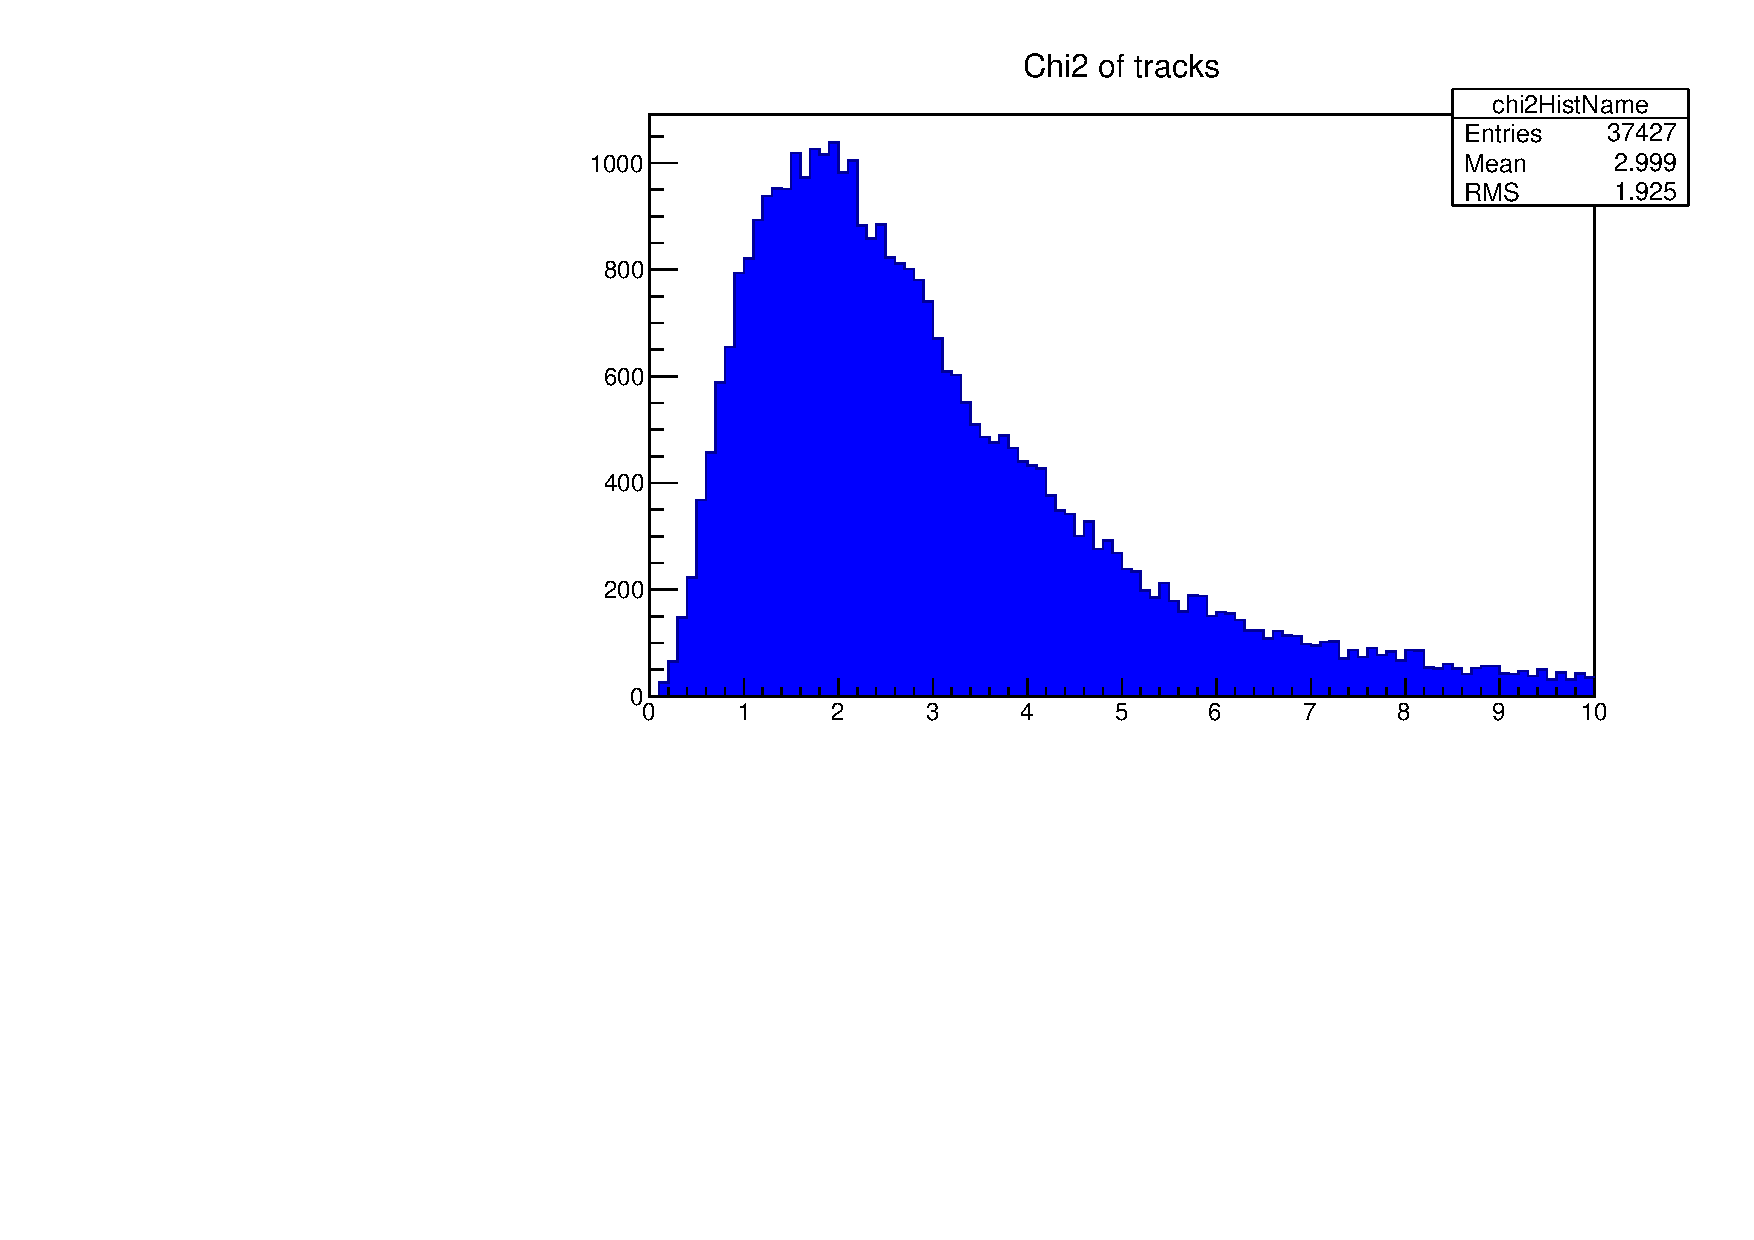
\includegraphics[width=0.9\linewidth]{pics/chi_new.pdf}\\
\tiny{\textbf{Not so perfect $\chi^{2}$/ndf.}}\\
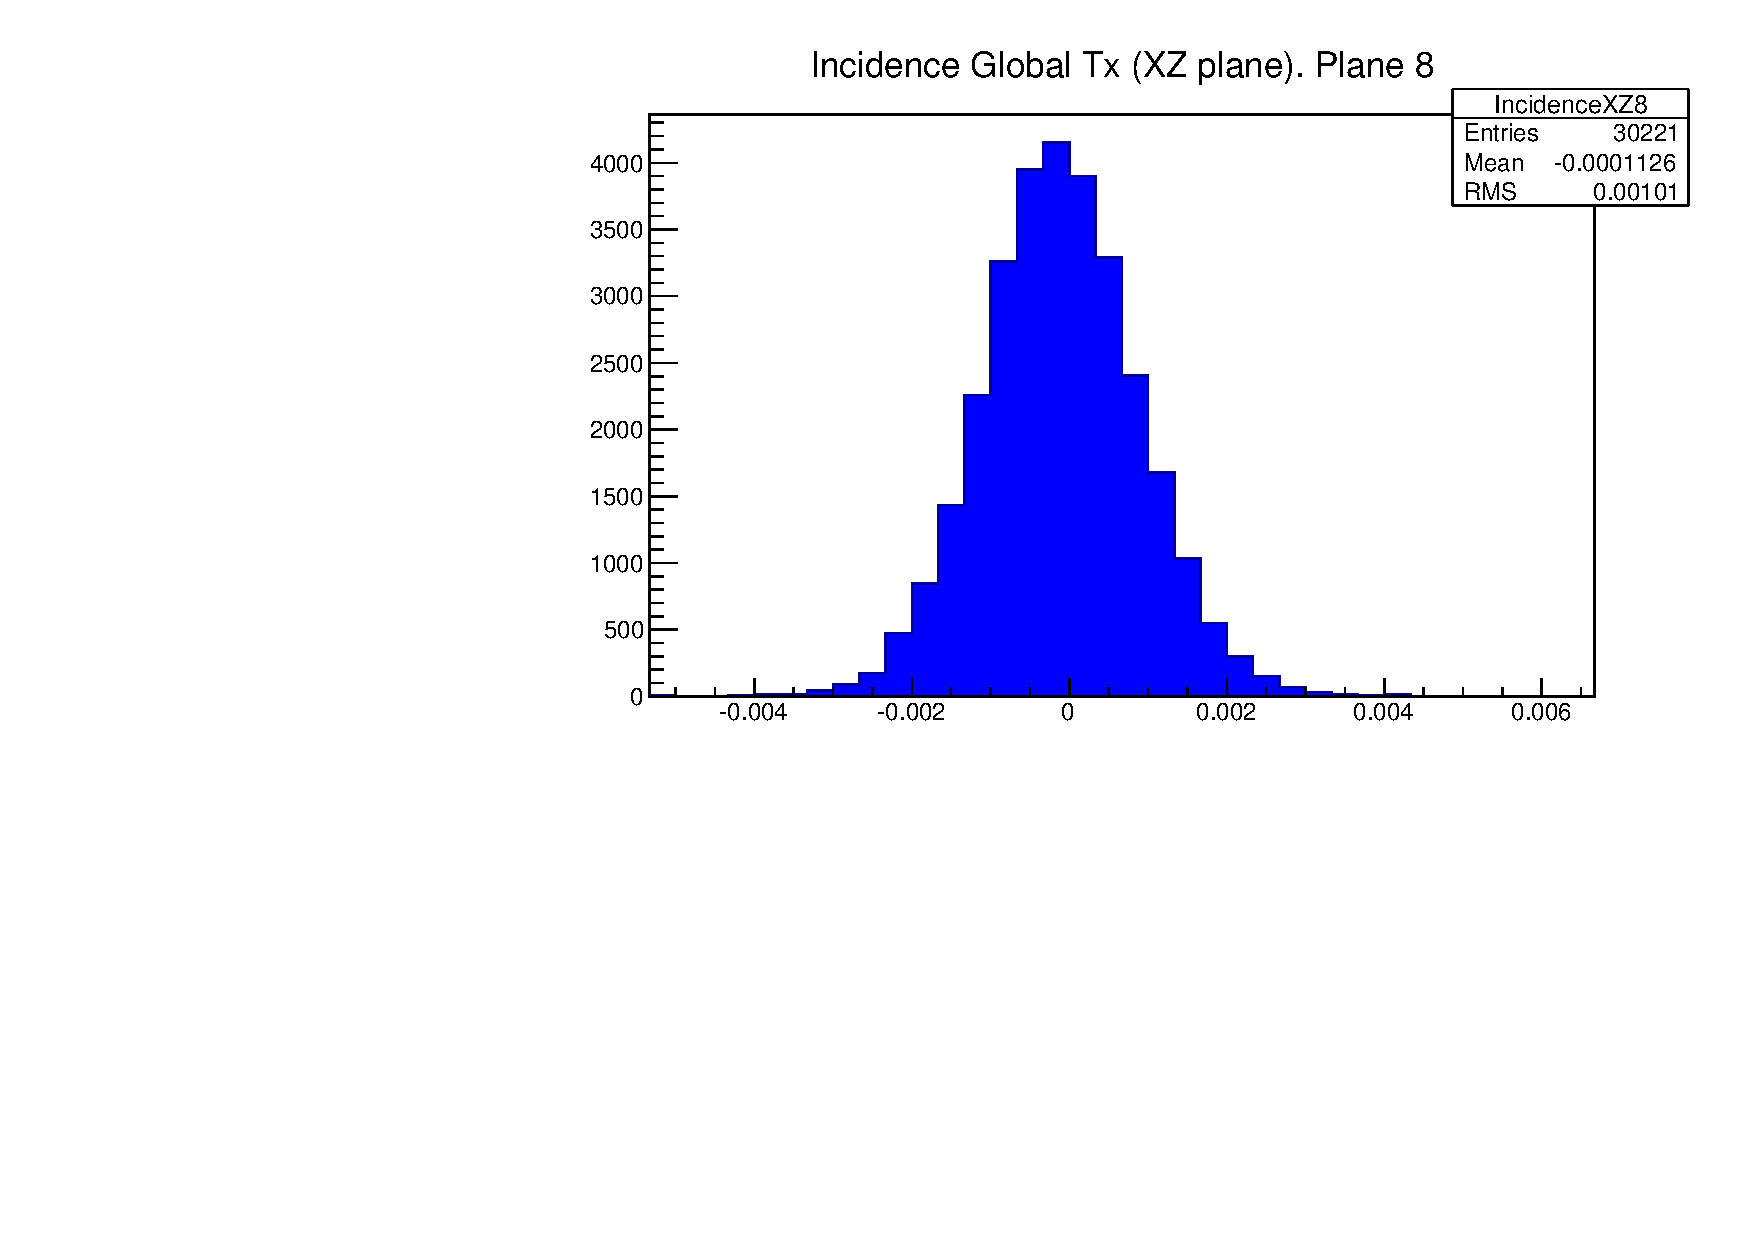
\includegraphics[width=0.9\linewidth]{pics/inc_new.pdf}\\
\tiny{\textbf{Incidence of track on DUT for local X axis. }}\\
\column{0.5\textwidth}
\centering
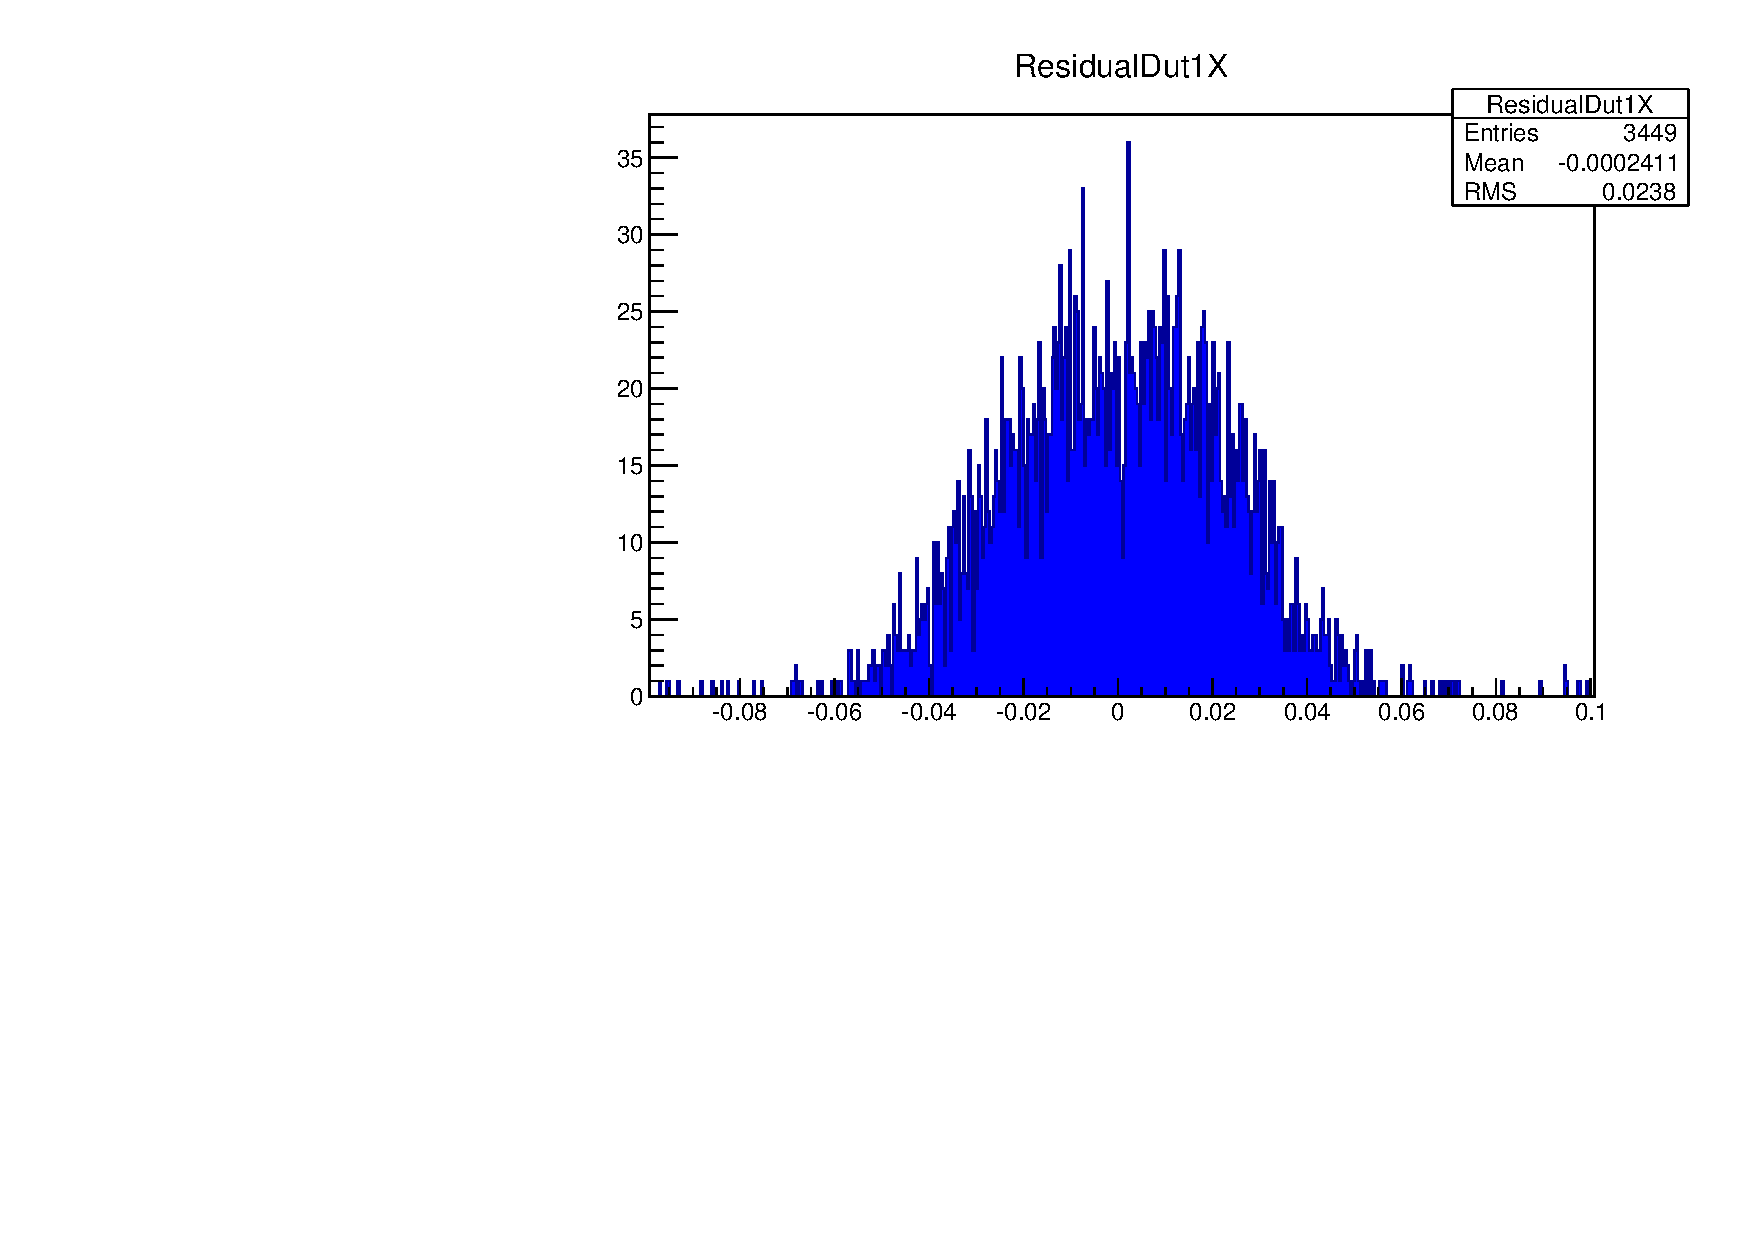
\includegraphics[width=0.9\linewidth]{pics/Res_new.pdf}\\ 
\tiny{\textbf{Residual on DUT for local X axis.}}

\tiny{
\vspace{10pt}
Some initial results from this weeks testbeam. \\
\vspace{10pt}
Reconstructed tracks are lower than expected at 0.5 per event (Expect about 1.5 in most cases).\\
\vspace{10pt}
Beam divergence is as expect and the residual RMS is dominated by the intrinsic error: $\sim$ 21 \si{\micro\metre\squared}.\\
\vspace{10pt}
However overall fit is still not perfect.
}

\end{columns}
\end{frame}

\end{document}
\section{Additional Information}
\subsection{EUDET/AIDA Pixel Beam Telescope}
\begin{frame}
\frametitle{ A Quick Detour: EUDET/AIDA Pixel Beam Telescope}
\begin{itemize}
\small{
\item 6 CMOS pixel detectors (18.4x18.4 \si{\micro\metre\squared}) $\rightarrow$ 1152 columns x 576 rows 2x1 $cm^2$.
\item Rolling shutter $\rightarrow$ continuous readout $\rightarrow$ 115.2 \si{\micro\second} integration time/frame.
\item Additional FEI4 device used for Region of Interest (ROI) and time stamping.
\item TLU and EUDAQ act as hard/soft layer for data acquisition.
\item EUTelescope is an advanced reconstruction framework for this setup, the latest workshop can be found \href{https://indico.desy.de/conferenceDisplay.py?ovw=True&confId=10685}{here}.
}
\end{itemize}
\begin{figure}
  \begin{columns}
        \column{.3\linewidth}
        \includegraphics[scale=0.03]{pics/setup.JPG}
        \label{fig:example left}
        \column{.6\linewidth}
        \caption{The mimosa sensors with a device under test (DUT).}
      \end{columns}
\end{figure}
\end{frame}

\begin{frame}
\frametitle{EUTelescope} 
\begin{itemize}
\item EUTelescope is a highly generic testbeam reconstruction and analysis framework.
\item It is a software package which is part of ILCsoft. A list of packages can be found \href{http://ilcsoft.desy.de/portal/software_packages/}{here}.
\item Relies on two packages for data structures and reconstruction.
 \begin{enumerate}
	\item Modular Analysis Reconstruction for the LINear Collider $\rightarrow$. \href{http://ilcsoft.desy.de/portal/software_packages/marlin/|}{Marlin}.
	\item Linear Collider Input Output $\rightarrow$ \href{http://ilcsoft.desy.de/portal/software_packages/lcio/}{LCIO}.
\end{enumerate}
\item On top of this additional software packages are used. 
\begin{enumerate}
	\item \href{http://www.desy.de/~blobel/mptalks.html}{Millepede}  $\rightarrow$ Algorithm designed for least squares fit problems with a large set of parameters.
	\item \href{ftp://root.cern.ch/root/doc/18Geometry.pdf}{TGeo} $\rightarrow$ A ROOT geometry package used to describe the small/large scale characteristics of the setup.
\end{enumerate}
\end{itemize}
The idea is to go from individual hit strips/pixels - or more complex - to the final reconstructed tracks. 
A general introduction is given \href{https://cds.cern.ch/record/2000969/files/AIDA-NOTE-2015-009.pdf}{here}.
\end{frame}

\subsection{Pattern Recognition}
\begin{frame}
\frametitle{Pattern Reconstruction}
You want to associate hits on each plane to a single track. This is more art than a science with many different procedures appropriate for different geometries and enviroments. 
\begin{columns}
\column{0.5\textwidth}
\begin{itemize}
\item Pattern Recognition comes with two regimes with GBL in EUTelescope.
 \begin{enumerate}
\small{
	\item Clustering: Extrapolate all hits to first plane and cluster (Useful if some planes have a low efficiency).
	\item Triplets Use both arms of the telescope to form triplets then link (Low fake rate. Recommended!).
}
\end{enumerate}
\item Both regimes work with arbitrary magnetic field.
\end{itemize}
\column{0.5\textwidth}
\begin{figure}
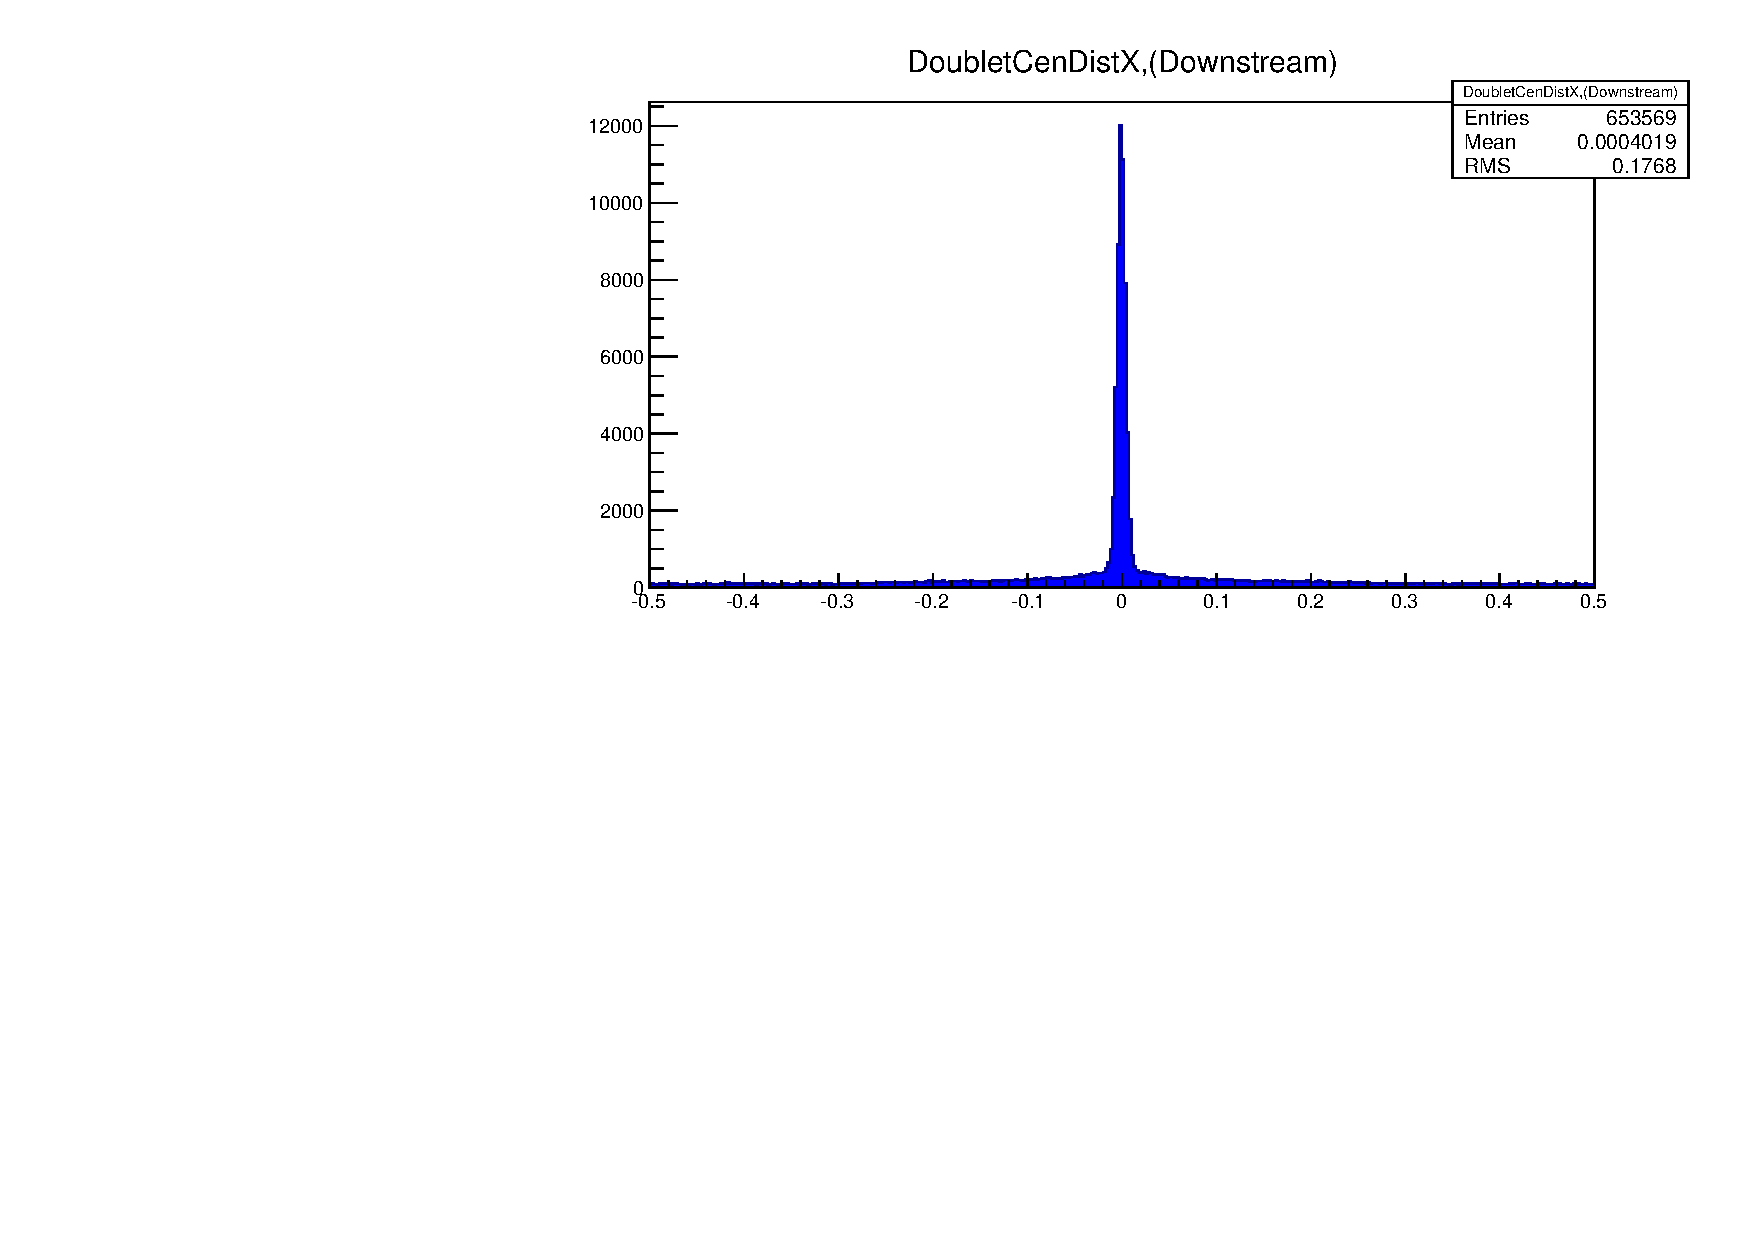
\includegraphics[scale=0.30]{pics/DoubletCenDist-442.pdf}	
\caption{\small{ Residual (mm) of prediction - measurement. A series of cuts is applied to determine signal from background.}}
\end{figure}
\end{columns}
\end{frame}

%\begin{frame}
%% This file was created by matlab2tikz.
%
%The latest updates can be retrieved from
%  http://www.mathworks.com/matlabcentral/fileexchange/22022-matlab2tikz-matlab2tikz
%where you can also make suggestions and rate matlab2tikz.
%
\definecolor{mycolor1}{rgb}{0.00000,0.44700,0.74100}%
%
\begin{tikzpicture}

\begin{axis}[%
%width=4.521in,
%height=3.566in,
width=3.3in,
height=2.8in,
at={(0.758in,0.481in)},
scale only axis,
xmin=0,
xmax=3,
xlabel={instrip position [strips 74.5 um]},
ymin=250,
ymax=350,
ylabel={mpv [mV]},
axis background/.style={fill=white},
title style={font=\bfseries},
title={mpv without pedestal substraction}
]
\addplot [color=mycolor1,only marks,mark=asterisk,mark options={solid},forget plot]
 plot [error bars/.cd, y dir = both, y explicit]
 table[row sep=crcr, y error plus index=2, y error minus index=3]{%
0.025	328.4129433	21.04355683	21.04355683\\
0.075	330.1934712	13.74228665	13.74228665\\
0.125	327.3348921	13.17078641	13.17078641\\
0.175	327.0707561	14.62318014	14.62318014\\
0.225	328.6506175	18.04569816	18.04569816\\
0.275	322.4987804	13.47272699	13.47272699\\
0.325	316.0177751	12.23881226	12.23881226\\
0.375	303.940173	13.4128864	13.4128864\\
0.425	292.1036442	13.61172539	13.61172539\\
0.475	281.5650039	9.979707699	9.979707699\\
0.525	266.4979761	6.64603907	6.64603907\\
0.575	271.6632253	9.635233772	9.635233772\\
0.625	285.7782389	7.77209775	7.77209775\\
0.675	298.055648	12.32673698	12.32673698\\
0.725	310.571005	10.77220652	10.77220652\\
0.775	315.0189865	13.68664645	13.68664645\\
0.825	327.1278621	19.9514166	19.9514166\\
0.875	322.7358733	14.40833842	14.40833842\\
0.925	321.9356295	13.81849046	13.81849046\\
0.975	327.0479318	17.79534336	17.79534336\\
1.025	326.7942199	21.22307195	21.22307195\\
1.075	325.7079256	13.17442163	13.17442163\\
1.125	329.1838776	19.92776657	19.92776657\\
1.175	325.9322407	13.30078989	13.30078989\\
1.225	319.6764966	11.3362512	11.3362512\\
1.275	318.0535249	13.02049123	13.02049123\\
1.325	316.1307186	17.14284888	17.14284888\\
1.375	305.6367823	15.88861375	15.88861375\\
1.425	288.4165597	11.0343911	11.0343911\\
1.475	279.6176186	6.58677415	6.58677415\\
1.525	264.3160117	7.532114431	7.532114431\\
1.575	271.2738445	9.440366803	9.440366803\\
1.625	286.1424228	8.407934037	8.407934037\\
1.675	305.1811668	13.89588557	13.89588557\\
1.725	316.0542609	15.89951197	15.89951197\\
1.775	320.802172	14.44281578	14.44281578\\
1.825	325.997343	15.11761964	15.11761964\\
1.875	329.6899353	16.0257406	16.0257406\\
1.925	325.3052423	15.90765752	15.90765752\\
1.975	331.1574404	14.55631136	14.55631136\\
2.025	330.4573065	19.47840344	19.47840344\\
2.075	328.8064408	18.72415366	18.72415366\\
2.125	327.1662737	15.82974734	15.82974734\\
2.175	326.226397	13.23947111	13.23947111\\
2.225	325.9292031	16.73345264	16.73345264\\
2.275	326.3815295	15.73112016	15.73112016\\
2.325	313.6452629	12.54754729	12.54754729\\
2.375	309.938131	11.96173373	11.96173373\\
2.425	291.1245048	9.548950662	9.548950662\\
2.475	274.3319899	8.527262123	8.527262123\\
2.525	265.3758565	9.002897232	9.002897232\\
2.575	271.4558906	10.63712	10.63712\\
2.625	285.8360472	10.55995537	10.55995537\\
2.675	303.3423682	10.45010684	10.45010684\\
2.725	312.845636	12.76735163	12.76735163\\
2.775	319.6869971	15.20865227	15.20865227\\
2.825	327.7006843	16.48111716	16.48111716\\
2.875	324.6705179	16.39830079	16.39830079\\
2.925	326.7228541	12.29428889	12.29428889\\
};
\end{axis}
\end{tikzpicture}%
%\end{frame}

%\begin{frame}
%% This file was created by matlab2tikz.
%
%The latest updates can be retrieved from
%  http://www.mathworks.com/matlabcentral/fileexchange/22022-matlab2tikz-matlab2tikz
%where you can also make suggestions and rate matlab2tikz.
%
\definecolor{mycolor1}{rgb}{0.00000,0.44700,0.74100}%
\definecolor{mycolor2}{rgb}{0.85000,0.32500,0.09800}%
\definecolor{mycolor3}{rgb}{0.92900,0.69400,0.12500}%
\definecolor{mycolor4}{rgb}{0.49400,0.18400,0.55600}%
\definecolor{mycolor5}{rgb}{0.46600,0.67400,0.18800}%
%
\begin{tikzpicture}

\begin{axis}[%
width=4.0in,
height=3.0in,
at={(0.758in,0.481in)},
scale only axis,
xmin=0,
xmax=3,
xlabel={instrip position [strips 74.5 um]},
ymin=0,
ymax=0.8,
ylabel={efficiency },
axis background/.style={fill=white}
]
\addplot [color=mycolor1,solid,forget plot]
  table[row sep=crcr]{%
-0.045	0.696759\\
0.005	0.678709\\
0.055	0.675\\
0.105	0.677725\\
0.155	0.683835\\
0.205	0.639752\\
0.255	0.600307\\
0.305	0.549659\\
0.355	0.502762\\
0.405	0.443291\\
0.455	0.364668\\
0.505	0.393819\\
0.555	0.451191\\
0.605	0.520581\\
0.655	0.5784\\
0.705	0.614907\\
0.755	0.643019\\
0.805	0.646526\\
0.855	0.659706\\
0.905	0.685368\\
0.955	0.686756\\
1.005	0.654914\\
1.055	0.678598\\
1.105	0.65188\\
1.155	0.630435\\
1.205	0.632865\\
1.255	0.616429\\
1.305	0.5625\\
1.355	0.477635\\
1.405	0.42071\\
1.455	0.355067\\
1.505	0.398739\\
1.555	0.453221\\
1.605	0.56184\\
1.655	0.626984\\
1.705	0.647558\\
1.755	0.664852\\
1.805	0.689956\\
1.855	0.688038\\
1.905	0.678098\\
1.955	0.707244\\
2.005	0.688302\\
2.055	0.683969\\
2.105	0.681048\\
2.155	0.675994\\
2.205	0.663166\\
2.255	0.59139\\
2.305	0.573273\\
2.355	0.477666\\
2.405	0.405303\\
2.455	0.375189\\
2.505	0.402941\\
2.555	0.461423\\
2.605	0.546828\\
2.655	0.595306\\
2.705	0.621155\\
2.755	0.684049\\
2.805	0.662695\\
2.855	0.670383\\
};
\addplot [color=mycolor2,solid,forget plot]
  table[row sep=crcr]{%
-2.02	1.78e-05\\
-1.98	0.00253566\\
-1.94	0.000310849\\
-1.9	0.00219024\\
-1.86	0.00438459\\
-1.82	0.00190235\\
-1.78	0.0021512\\
-1.74	0.00351325\\
-1.7	0.00128908\\
-1.66	0.00378907\\
-1.62	0.00224072\\
-1.58	0.00354153\\
-1.54	0.00190416\\
-1.5	0.00230187\\
-1.46	0.00408934\\
-1.42	0.00473186\\
-1.38	0.00480461\\
-1.34	0.00436545\\
-1.3	0.00404606\\
-1.26	0.00527623\\
-1.22	0.0056872\\
-1.18	0.00736236\\
-1.14	0.0028125\\
-1.1	0.00608974\\
-1.06	0.00663088\\
-1.02	0.00783208\\
-0.98	0.00792393\\
-0.94	0.00839291\\
-0.9	0.00876095\\
-0.86	0.0112747\\
-0.82	0.0145847\\
-0.78	0.0187462\\
-0.74	0.0242734\\
-0.7	0.0425395\\
-0.66	0.0574676\\
-0.62	0.0861076\\
-0.58	0.121056\\
-0.54	0.169787\\
-0.5	0.271621\\
-0.46	0.357345\\
-0.42	0.449527\\
-0.38	0.524664\\
-0.34	0.568444\\
-0.3	0.630563\\
-0.26	0.638734\\
-0.22	0.663507\\
-0.18	0.667734\\
-0.14	0.680937\\
-0.1	0.672115\\
-0.06	0.684244\\
-0.02	0.691103\\
0.02	0.692235\\
0.06	0.680448\\
0.1	0.65801\\
0.14	0.673974\\
0.18	0.653773\\
0.22	0.619238\\
0.26	0.604919\\
0.3	0.539478\\
0.34	0.47616\\
0.38	0.362996\\
0.42	0.288474\\
0.46	0.204697\\
0.5	0.134166\\
0.54	0.0890217\\
0.58	0.0574132\\
0.62	0.0429212\\
0.66	0.0215154\\
0.7	0.0214753\\
0.74	0.0117939\\
0.78	0.014218\\
0.82	0.00672215\\
0.86	0.008125\\
0.9	0.00833333\\
0.94	0.00599937\\
0.98	0.0037594\\
1.02	0.00792393\\
1.06	0.00590612\\
1.1	0.00406758\\
1.14	0.00720326\\
1.18	0.00919467\\
1.22	0.00368777\\
1.26	0.00542958\\
1.3	0.00483403\\
1.34	0.00442059\\
1.38	0.00288092\\
1.42	0.00289762\\
1.46	0.00539511\\
1.5	0.00328839\\
1.54	0.00251651\\
1.58	0.00315457\\
1.62	0.0044843\\
1.66	0.00343\\
1.7	0.00373483\\
1.74	0.00217256\\
1.78	0.00221169\\
1.82	0.000320102\\
1.86	0.001875\\
1.9	0.00224359\\
1.94	0.000947269\\
};
\addplot [color=mycolor3,solid,forget plot]
  table[row sep=crcr]{%
-1.02	1.78e-05\\
-0.98	0.00253566\\
-0.94	0.000310849\\
-0.9	0.00219024\\
-0.86	0.00438459\\
-0.82	0.00190235\\
-0.78	0.0021512\\
-0.74	0.00351325\\
-0.7	0.00128908\\
-0.66	0.00378907\\
-0.62	0.00224072\\
-0.58	0.00354153\\
-0.54	0.00190416\\
-0.5	0.00230187\\
-0.46	0.00408934\\
-0.42	0.00473186\\
-0.38	0.00480461\\
-0.34	0.00436545\\
-0.3	0.00404606\\
-0.26	0.00527623\\
-0.22	0.0056872\\
-0.18	0.00736236\\
-0.14	0.0028125\\
-0.1	0.00608974\\
-0.0600000000000001	0.00663088\\
-0.02	0.00783208\\
0.02	0.00792393\\
0.0600000000000001	0.00839291\\
0.1	0.00876095\\
0.14	0.0112747\\
0.18	0.0145847\\
0.22	0.0187462\\
0.26	0.0242734\\
0.3	0.0425395\\
0.34	0.0574676\\
0.38	0.0861076\\
0.42	0.121056\\
0.46	0.169787\\
0.5	0.271621\\
0.54	0.357345\\
0.58	0.449527\\
0.62	0.524664\\
0.66	0.568444\\
0.7	0.630563\\
0.74	0.638734\\
0.78	0.663507\\
0.82	0.667734\\
0.86	0.680937\\
0.9	0.672115\\
0.94	0.684244\\
0.98	0.691103\\
1.02	0.692235\\
1.06	0.680448\\
1.1	0.65801\\
1.14	0.673974\\
1.18	0.653773\\
1.22	0.619238\\
1.26	0.604919\\
1.3	0.539478\\
1.34	0.47616\\
1.38	0.362996\\
1.42	0.288474\\
1.46	0.204697\\
1.5	0.134166\\
1.54	0.0890217\\
1.58	0.0574132\\
1.62	0.0429212\\
1.66	0.0215154\\
1.7	0.0214753\\
1.74	0.0117939\\
1.78	0.014218\\
1.82	0.00672215\\
1.86	0.008125\\
1.9	0.00833333\\
1.94	0.00599937\\
1.98	0.0037594\\
2.02	0.00792393\\
2.06	0.00590612\\
2.1	0.00406758\\
2.14	0.00720326\\
2.18	0.00919467\\
2.22	0.00368777\\
2.26	0.00542958\\
2.3	0.00483403\\
2.34	0.00442059\\
2.38	0.00288092\\
2.42	0.00289762\\
2.46	0.00539511\\
2.5	0.00328839\\
2.54	0.00251651\\
2.58	0.00315457\\
2.62	0.0044843\\
2.66	0.00343\\
2.7	0.00373483\\
2.74	0.00217256\\
2.78	0.00221169\\
2.82	0.000320102\\
2.86	0.001875\\
2.9	0.00224359\\
2.94	0.000947269\\
};
\addplot [color=mycolor4,solid,forget plot]
  table[row sep=crcr]{%
-0.02	1.78e-05\\
0.02	0.00253566\\
0.0600000000000001	0.000310849\\
0.1	0.00219024\\
0.14	0.00438459\\
0.18	0.00190235\\
0.22	0.0021512\\
0.26	0.00351325\\
0.3	0.00128908\\
0.34	0.00378907\\
0.38	0.00224072\\
0.42	0.00354153\\
0.46	0.00190416\\
0.5	0.00230187\\
0.54	0.00408934\\
0.58	0.00473186\\
0.62	0.00480461\\
0.66	0.00436545\\
0.7	0.00404606\\
0.74	0.00527623\\
0.78	0.0056872\\
0.82	0.00736236\\
0.86	0.0028125\\
0.9	0.00608974\\
0.94	0.00663088\\
0.98	0.00783208\\
1.02	0.00792393\\
1.06	0.00839291\\
1.1	0.00876095\\
1.14	0.0112747\\
1.18	0.0145847\\
1.22	0.0187462\\
1.26	0.0242734\\
1.3	0.0425395\\
1.34	0.0574676\\
1.38	0.0861076\\
1.42	0.121056\\
1.46	0.169787\\
1.5	0.271621\\
1.54	0.357345\\
1.58	0.449527\\
1.62	0.524664\\
1.66	0.568444\\
1.7	0.630563\\
1.74	0.638734\\
1.78	0.663507\\
1.82	0.667734\\
1.86	0.680937\\
1.9	0.672115\\
1.94	0.684244\\
1.98	0.691103\\
2.02	0.692235\\
2.06	0.680448\\
2.1	0.65801\\
2.14	0.673974\\
2.18	0.653773\\
2.22	0.619238\\
2.26	0.604919\\
2.3	0.539478\\
2.34	0.47616\\
2.38	0.362996\\
2.42	0.288474\\
2.46	0.204697\\
2.5	0.134166\\
2.54	0.0890217\\
2.58	0.0574132\\
2.62	0.0429212\\
2.66	0.0215154\\
2.7	0.0214753\\
2.74	0.0117939\\
2.78	0.014218\\
2.82	0.00672215\\
2.86	0.008125\\
2.9	0.00833333\\
2.94	0.00599937\\
2.98	0.0037594\\
3.02	0.00792393\\
3.06	0.00590612\\
3.1	0.00406758\\
3.14	0.00720326\\
3.18	0.00919467\\
3.22	0.00368777\\
3.26	0.00542958\\
3.3	0.00483403\\
3.34	0.00442059\\
3.38	0.00288092\\
3.42	0.00289762\\
3.46	0.00539511\\
3.5	0.00328839\\
3.54	0.00251651\\
3.58	0.00315457\\
3.62	0.0044843\\
3.66	0.00343\\
3.7	0.00373483\\
3.74	0.00217256\\
3.78	0.00221169\\
3.82	0.000320102\\
3.86	0.001875\\
3.9	0.00224359\\
3.94	0.000947269\\
};
\addplot [color=mycolor5,solid,forget plot]
  table[row sep=crcr]{%
0.98	1.78e-05\\
1.02	0.00253566\\
1.06	0.000310849\\
1.1	0.00219024\\
1.14	0.00438459\\
1.18	0.00190235\\
1.22	0.0021512\\
1.26	0.00351325\\
1.3	0.00128908\\
1.34	0.00378907\\
1.38	0.00224072\\
1.42	0.00354153\\
1.46	0.00190416\\
1.5	0.00230187\\
1.54	0.00408934\\
1.58	0.00473186\\
1.62	0.00480461\\
1.66	0.00436545\\
1.7	0.00404606\\
1.74	0.00527623\\
1.78	0.0056872\\
1.82	0.00736236\\
1.86	0.0028125\\
1.9	0.00608974\\
1.94	0.00663088\\
1.98	0.00783208\\
2.02	0.00792393\\
2.06	0.00839291\\
2.1	0.00876095\\
2.14	0.0112747\\
2.18	0.0145847\\
2.22	0.0187462\\
2.26	0.0242734\\
2.3	0.0425395\\
2.34	0.0574676\\
2.38	0.0861076\\
2.42	0.121056\\
2.46	0.169787\\
2.5	0.271621\\
2.54	0.357345\\
2.58	0.449527\\
2.62	0.524664\\
2.66	0.568444\\
2.7	0.630563\\
2.74	0.638734\\
2.78	0.663507\\
2.82	0.667734\\
2.86	0.680937\\
2.9	0.672115\\
2.94	0.684244\\
2.98	0.691103\\
3.02	0.692235\\
3.06	0.680448\\
3.1	0.65801\\
3.14	0.673974\\
3.18	0.653773\\
3.22	0.619238\\
3.26	0.604919\\
3.3	0.539478\\
3.34	0.47616\\
3.38	0.362996\\
3.42	0.288474\\
3.46	0.204697\\
3.5	0.134166\\
3.54	0.0890217\\
3.58	0.0574132\\
3.62	0.0429212\\
3.66	0.0215154\\
3.7	0.0214753\\
3.74	0.0117939\\
3.78	0.014218\\
3.82	0.00672215\\
3.86	0.008125\\
3.9	0.00833333\\
3.94	0.00599937\\
3.98	0.0037594\\
4.02	0.00792393\\
4.06	0.00590612\\
4.1	0.00406758\\
4.14	0.00720326\\
4.18	0.00919467\\
4.22	0.00368777\\
4.26	0.00542958\\
4.3	0.00483403\\
4.34	0.00442059\\
4.38	0.00288092\\
4.42	0.00289762\\
4.46	0.00539511\\
4.5	0.00328839\\
4.54	0.00251651\\
4.58	0.00315457\\
4.62	0.0044843\\
4.66	0.00343\\
4.7	0.00373483\\
4.74	0.00217256\\
4.78	0.00221169\\
4.82	0.000320102\\
4.86	0.001875\\
4.9	0.00224359\\
4.94	0.000947269\\
};
\end{axis}
\end{tikzpicture}%
%\end{frame}
\subsection{List of Examples}
\begin{frame}
\frametitle{The Fitter in Action}
EUTelescope is a collaborative effort first and foremost and to that end many working examples have been created to aid further analysis. The full analysis chain is described for each example and works from installation (Data on DESY AFS).  Brief Manual \href{https://github.com/AlexanderMorton/GBLManuel/blob/master/thesis.pdf}{here}
\begin{description} 
\item[noDUTExample] \small{This example demostrates the use of the fitter with magnetic fields and varying beam energies}.
\item[Quad] \small{Quad module with reference DUT at the DESY testbeam }.
\item[QuadSLAC]  \small{Quad module and reference DUT at the SLAC testbeam}.
\item[Pixels] \small{High radiation length enviroment using the gear file to describe dead material. Two APIX devices at DESY testbeam.}
\item[mappingAPIX] \small{Two APIX DUTs using the mapping processor between channel number and geometric cluster position.}
\item[mappingAPIXSLAC] \small{This is the same as the other mapping example but at SLAC and with highly irradiated sensors.}
\item[SCT] \small{Strip example which has been used for efficiency measurements.}
\item[StripAlibava] \small{ATLAS12 strip device using the alibava system as readout.}
\item[X0] \small{The use of the kink angle estimation is demonstrated here.}
\end{description} 
\end{frame}
\subsection{Reconstruction within EUTelescope}
\begin{frame}
\frametitle{Reconstruction in a Nutshell}
\begin{columns}
\column{0.5\textwidth}
\begin{figure}
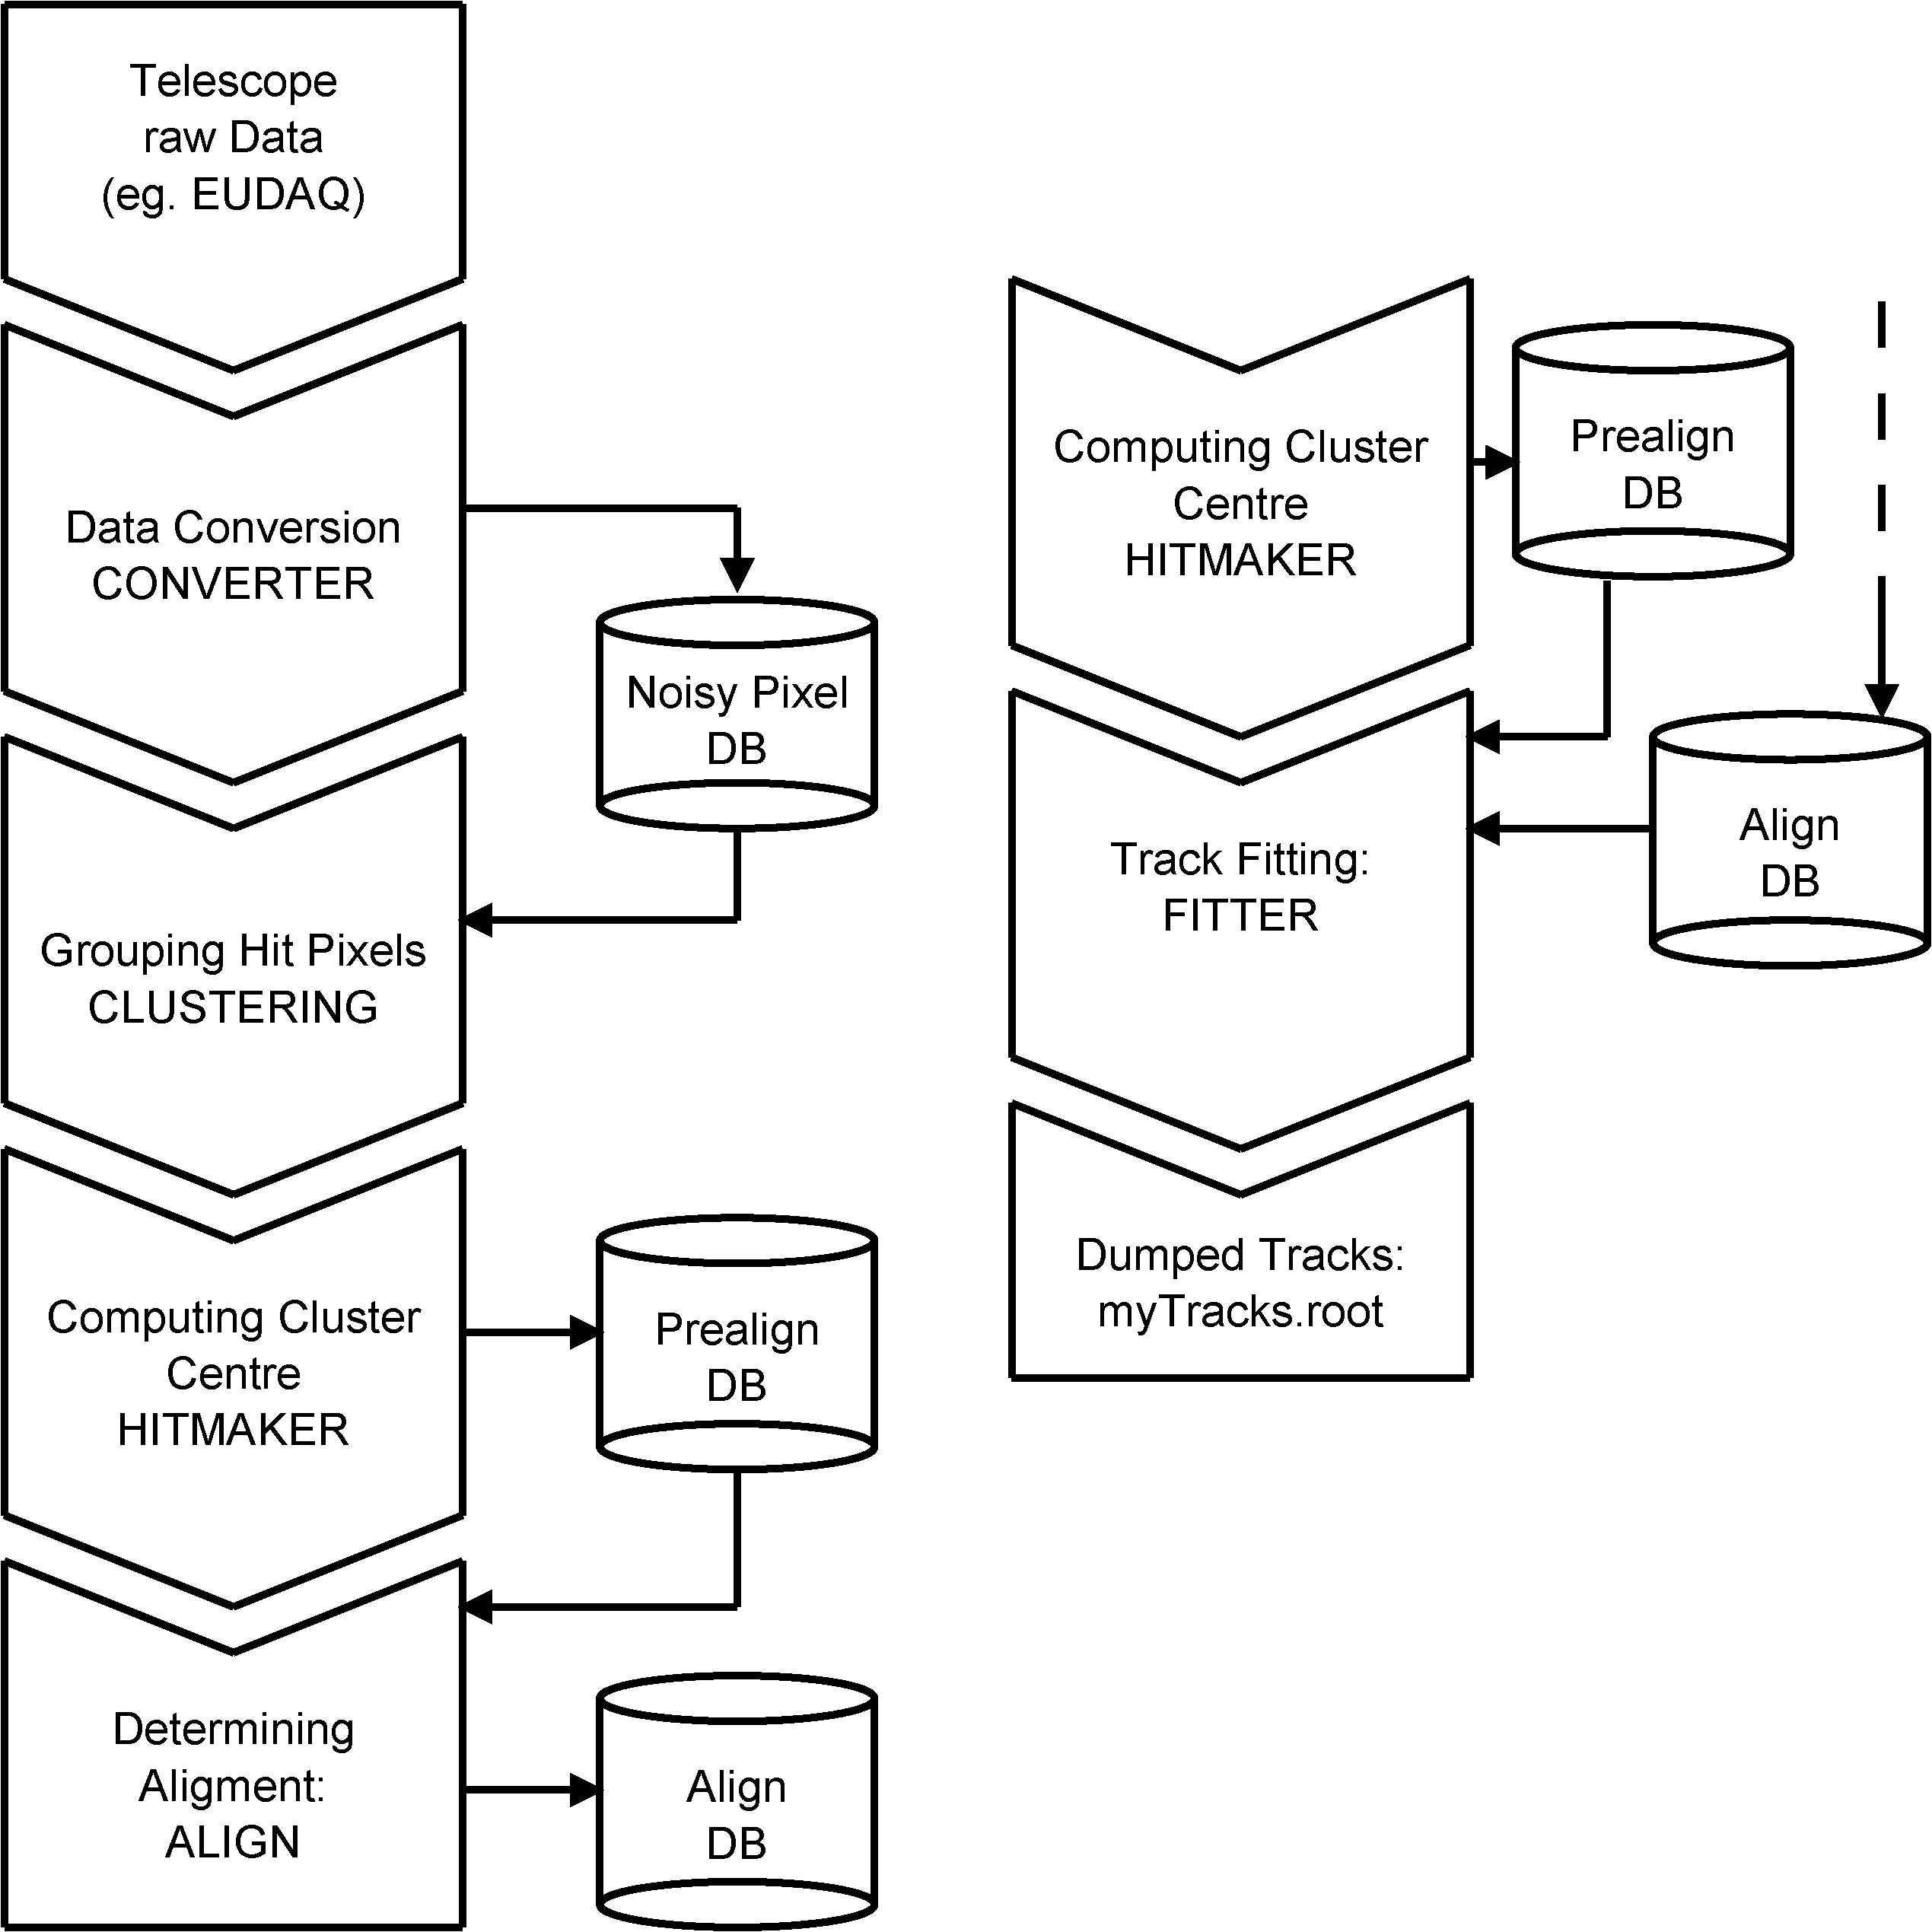
\includegraphics[scale=0.13]{pics/EUTelFullRecoChain.pdf}
\caption{\tiny{A typical reconstruction chain. Different processors can reconstruct the clusters/hits/track in different ways depending on the analysis.}}
\end{figure}
\column{0.5\textwidth}
Reconstruction comes in a series of steps with track fitting coming last in the chain. 
\begin{itemize}
\tiny{
\item Converter: Takes unique output from readout system and creates an LCIO file with the required format. (Can combine telescope and DUT data further down the chain).
\pause
\item Clustering: TGeo used here to relate fired channel number to a geometric pixel (Many different types of cluster can be classified using different techniques).
\pause
\item Hitmaker: Relates clusters to a single hit position with intrinsic measurement errors.
\pause
\item Pre/Full Alignment: Determines physical position of sensors. Different track models and alignment parameterizations can be used. However all methods depend on Millepede for least squares fitting for local/global parameters.
\pause
\item Tracking: The most likely track given initial assumptions is deduced, the final tracks are output in lcio/root formats.
}
\end{itemize}
\end{columns}
\end{frame}

\subsection{Track Creation}
\begin{frame}
\frametitle{Track Fitting with GBL Algorithm}
The GBL algorithm has easy interfaces to include the needed information for a track fit and recovering the fit parameters. This information would be needed in any tracking situation and a quick introduction is presented now: \\
\textbf{The five fold way}
\begin{enumerate}
\item \small{ Need to link discretized points to form a full trajectory. Figure \ref{Scat} shows the specific setup for EUTelescope.}
\item \small{The trajectory must contain measurements with errors. Figure \ref{Scat} \textcolor{red}{Red Points}.}
\item \small{ Points which model scattering have kink angles and errors added. Figure \ref{Scat} \textcolor{orange}{Orange Points}.}
\item \small{ Global derivatives which relate motions of the sensors with local frame residuals are added for alignment.}
\item \small{\textit{If needed: Local derivatives are added to determine parameters which relate to the track's residual on certain planes}.}
\end{enumerate}
\end{frame}


\end{document} 

\begin{frame}
\frametitle{Track Reconstruction in EUTelescope}
\small{
\begin{itemize}
\item Deterministic Annealing Filter $\rightarrow$ DAF. 
\begin{enumerate}
\small{
\item Designed to include multiple measurements in a single fit.
\item Scattering information is added as additional uncertainty in covariance matrix.
\item Does not allow tracking with curved tracks (Magnetic fields). 
\item Updates are coming! Watch this space. 
}
\end{enumerate}
\item  General Broken Lines Algorithm $\rightarrow$ \href{http://www.desy.de/~kleinwrt/GBL/doc/cpp/html/index.html}{GBL}.
\begin{enumerate}
\small{
\item Global fit performed with fit parameters: $(q/p,o_{1},o_{2},o_{3})$ $\rightarrow$ curvature and offsets.
\item Scattering information is included in fit in the form of kink angles. Useful for X0 measurements.
\item Fitting with arbitrary magnetic fields.
}
\item Algorithm implemented in C++.
\end{enumerate}
\end{itemize}
A very preliminary comparison of the current DAFFitter and GBL can be found \href{https://github.com/AlexanderMorton/GBLManuel/blob/master/RyanNelsonSummerPPEReport.pdf}{here}. 
}
\end{frame}

\subsection{Track Fitting with GBL in EUTelescope}
\begin{frame}
\frametitle{Track Fitting with GBL Algorithm}
\begin{itemize}
\item The GBL package has interfaces to include the needed information for a track fit and recovering the fit parameters.
\item The package requires additional software to work within EUTelescope. 
\begin{enumerate}
	\item Millepede  $\rightarrow$ Algorithm designed for least squares fit problems with a large set of parameters.
	\item TGeo $\rightarrow$ A ROOT geometry package used to describe the small/large scale characteristics of the setup.
	\item Marlin $\rightarrow$ Used for event by event processing. 
	\item LCIO $\rightarrow$ Data model. 
\end{enumerate}
\end{itemize}
\vspace{10pt}
\textbf{A single track can be constructed in 4 steps...} 
\end{frame}